\documentclass{article}
\usepackage{iclr2026_conference,times}
\input{math_commands.tex}
\usepackage{booktabs}
\usepackage{graphicx}
\usepackage{amsmath}
\usepackage{amssymb}
\usepackage{amsthm}
\usepackage{xcolor}
\usepackage{url}
\usepackage[
  colorlinks=false,
  pdfborder={0 0 1},
  citebordercolor={1 0.48 0},
  linkbordercolor={0 0.45 1},
  urlbordercolor={0 0.65 0.25}
]{hyperref}

\newtheorem{proposition}{Proposition}
\newtheorem{lemma}{Lemma}
\newtheorem{theorem}{Theorem}
\newcommand{\method}{RC-RET}
\newcommand{\actionset}{\mathcal{A}}
\newcommand{\latent}{\theta}
\newcommand{\energy}{E}
\newcommand{\risk}{\rho}

\title{Risk-Calibrated Relational Energy Transformers for Contact-Rich Action Selection: A Strong-Revise MuJoCo Study}
\author{Anonymous Authors}

\begin{document}
\maketitle

\begin{abstract}
Selecting one action from a finite set of contact-rich manipulation primitives is a deceptively difficult setting for learned policies: the best action depends not only on local progress toward the target, but also on the relative risk profile of all feasible alternatives under latent mass, friction, obstacle, and actuation shifts.  This paper rebuilds Energy Transformer Action Selection into a real CPU-only MuJoCo/PyTorch evidence package.  We introduce a risk-calibrated relational energy transformer (\method) that scores candidate push primitives using set context, branch-risk summaries, and a predefined safety shield.  The frozen protocol evaluates 11,520 paired main episodes and 2,112 ablation episodes over ten stress splits, twelve main methods, and eleven ablation variants.  The result is useful but not ICLR-main ready.  \method{} is near robust branch scoring, improves safety relative to unshielded learned baselines, and its feasibility objective is necessary; however, it does not clear the success gate against MLP energy, Deep Sets, robust MPC, or the oracle, and narrow-clearance cases expose a hard limitation of the finite action library.  We therefore report the honest terminal decision: \textbf{STRONG\_REVISE}.  The contribution is a reproducible, hostile-review-ready negative result and a clearer map of what an action-set energy method must prove before it deserves a main-conference claim.
\end{abstract}

\section{Introduction}

Many robot policies decode a single next action.  That design is convenient, but in contact-rich manipulation the robot often faces a small manifold of plausible primitive actions: push slightly left or right of an obstacle, take a longer but safer path, choose an aggressive low-friction primitive, or accept a conservative action that leaves more residual distance.  An action selector should therefore reason over the action set, not only over each candidate independently.  This intuition is shared by energy-based imitation methods \citep{lecun2006tutorial,florence2022implicit}, set models \citep{zaheer2017deep,lee2019set}, transformer policies \citep{vaswani2017attention,zhao2023learning}, diffusion policies \citep{chi2023diffusion}, and model-based control methods \citep{williams2017mppi,chua2018pets}.

The original version of this paper had the right research taste but the wrong evidence.  It framed action selection as energy-ranked feasible action manifolds, but its evidence was synthetic and its transformer mechanism was not isolated.  A subsequent v4 rebuild replaced the synthetic scaffold with a real MuJoCo/PyTorch pushing benchmark \citep{todorov2012mujoco}; nevertheless, the learned transformer failed to consistently beat MLP energy, nominal MPC, or robust worst-case MPC.  The correct response is not to make the writing prettier.  The correct response is to make the claim harder to satisfy.

This v5 paper does that.  We rebuild the method as a risk-calibrated relational energy transformer (\method).  \method{} is not ``a transformer because transformers are fashionable.''  It is a set scorer with three specific mechanisms.  First, candidate actions are represented as a permutation-equivariant action set.  Second, each candidate receives branch-risk summaries under latent mass and friction hypotheses.  Third, a safety shield filters actions whose modeled branch clearances violate a predefined margin.  The transformer is used as residual calibration over a robust-risk frontier, not as an ungrounded black box.

We then freeze a hostile protocol: ten stress splits, eight seeds, twelve episodes per split/seed, twelve methods, eleven ablations, 63 candidate actions per episode, paired bootstrap intervals, sign-flip tests, oracle regret, violation rates, and explicit negative cases.  The protocol is CPU-only and RAM-light.  It is also deliberately unforgiving: MLP energy, shielded MLP, Deep Sets, robust MPC, branch-CVaR scoring, and the true MuJoCo rollout oracle are all included.  A method cannot become submission-ready merely by beating random or geometric selection.

\paragraph{Outcome.}
The final decision is \textbf{STRONG\_REVISE}.  \method{} is close to robust branch scoring and safer than several unshielded learned baselines.  It avoids some violation failures of MLP and Deep Sets.  But it does not win the aggregate success gate: compared with robust MPC, its aggregate success delta is $-0.0042$; compared with MLP, $-0.0240$; compared with Deep Sets, $-0.0437$; compared with the oracle, $-0.1615$.  In narrow-clearance scenes, \method{} reaches zero success under the frozen success radius while the oracle still finds a small nonzero feasible region.  These results do not support an ICLR-main-ready positive claim.

\paragraph{Contributions.}
This paper contributes:
\begin{itemize}
\item A real MuJoCo/PyTorch action-set selection benchmark with 11,520 frozen main rows and 2,112 ablation rows.
\item A stronger action-set method, \method, that combines branch-risk features, permutation-equivariant scoring, residual transformer calibration, and a predefined safety shield.
\item A formal problem setup, equivariance proposition, regret decomposition, safety-shield lemma, and negative identifiability theorem.
\item A hostile empirical protocol with strong baselines, stress tests, ablations, uncertainty reporting, and explicit failure cases.
\item An honest terminal decision: \textbf{STRONG\_REVISE}, with evidence that the current method is not yet ICLR-main-ready.
\end{itemize}

\section{Why the v4 Thesis Failed}

The v4 benchmark was valuable because it replaced synthetic tables with real MuJoCo rollout labels.  It also revealed a structural weakness.  Candidate tokens contained strong per-action features, including geometric progress and nominal rollout energy.  A small transformer over those tokens therefore had little opportunity to prove that self-attention mattered.  The MLP baseline received nearly the same decisive information, and robust MPC could directly evaluate branch outcomes.  Under that evidence, the transformer architecture was not the contribution.

The failure is instructive.  In finite action-set selection, set context can matter only when the selected action depends on relative structure: which alternatives form the safety frontier, which candidates dominate under different latent parameters, and how risk should be traded against progress when no candidate is uniformly best.  If each candidate can be scored independently with nearly sufficient features, a transformer is decorative.  The v5 plan therefore forces the method to expose and test a stronger mechanism:
\begin{enumerate}
\item Branch-risk summaries must be available and fairly shared with non-transformer baselines.
\item The set model must be compared against Deep Sets, not only against an MLP.
\item Safety calibration must be explicit and measured.
\item The final protocol must include splits where robust control is expected to be strong, not just splits where a learned scorer might look good.
\end{enumerate}

\section{Problem Setup}

We consider a finite action-set selection problem for contact-rich manipulation.  A state $s$ contains observed puck position, target position, obstacle position, and candidate primitive geometry.  Hidden physical parameters $\latent \in \Theta$ include mass, friction, and actuation perturbation.  The robot receives a finite candidate set
\[
  \actionset(s) = \{a_1,\ldots,a_K\},
\]
where each $a_i$ is a push primitive parameterized by approach angle, lateral offset, and push distance.  In the v5 benchmark, $K=63$.

For candidate $a_i$, simulator rollout under latent parameter $\latent$ produces final puck position $x_T(s,a_i,\latent)$, effort $u(s,a_i,\latent)$, and a binary obstacle/contact violation $v(s,a_i,\latent)$.  The true rollout energy is
\[
  \energy(s,a_i,\latent)
  =
  \|x_T(s,a_i,\latent)-x^\star(s)\|_2
  + \lambda_u u(s,a_i,\latent)
  + \lambda_v v(s,a_i,\latent),
\]
where $x^\star(s)$ is the target.  In experiments $\lambda_u=0.03$ and $\lambda_v=0.32$.  Success is separately measured as final distance below $0.075$ with no violation.

The selector chooses
\[
  \pi(s,\actionset) \in \arg\min_{a_i \in \actionset(s)} \widehat{\energy}(s,\actionset,a_i),
\]
where $\widehat{\energy}$ may depend on the full action set.  The oracle selector has access to the true rollout energies for the evaluation latent parameter and chooses $\arg\min_i \energy(s,a_i,\latent)$.  No learned method is expected to dominate this oracle; the oracle is an upper bound used to measure regret.

\paragraph{Risk branches.}
At inference, branch summaries are computed under a small modeled branch set $\mathcal{B}$ containing low-friction, nominal, heavy-object, and high-friction hypotheses.  For candidate $a_i$, the branch-risk feature vector includes mean branch energy, max branch energy, branch-energy standard deviation, CVaR-like tail mean, mean and max branch distance, max modeled violation, minimum branch clearance, nominal energy, nominal violation, and branch energy gap.  These features are shared with the MLP, Deep Sets, and branch-score baselines where appropriate.

\paragraph{What can be claimed.}
A learned action-set method is interesting only if it improves the realized tradeoff among success, regret, and violations relative to strong baselines.  Beating random or geometric selection is not enough.  This distinction drives all terminal gates.

\section{\method: Risk-Calibrated Relational Energy Transformer}

\subsection{Candidate Manifold}

Each episode generates a library of 63 candidate pushes.  The base direction points from puck to target.  We perturb the direction by seven angular offsets, apply three lateral offsets, and scale the distance by three factors.  This creates short, long, left-biased, center, and right-biased primitives.  The library remains small enough for CPU-only MuJoCo rollouts but large enough to expose obstacle-avoidance and conservatism tradeoffs.

The same candidate library is used for all methods.  This is essential.  Otherwise a learned method could appear better simply because it receives easier candidates.

\subsection{Token Features}

For candidate $a_i$, the feature vector contains:
\begin{itemize}
\item Local geometry: relative angle, offset, distance, initial target distance, geometric final distance, geometric progress, obstacle clearance, target-obstacle distance, puck-obstacle distance, and squared distance.
\item Branch-risk summaries: mean, max, standard deviation, and tail mean of branch energies; branch distance summaries; maximum branch violation; minimum branch clearance; nominal energy; nominal violation; branch energy gap; clearance margin.
\item Set-relative ranks: geometric rank, branch-CVaR rank, worst-branch rank, and clearance rank.
\end{itemize}
The rank features are simple but important: they make each token aware of where it sits on the candidate frontier.

\subsection{Architecture}

\method{} maps a standardized candidate-feature matrix $X \in \mathbb{R}^{K \times d}$ to an energy score and violation logit for every candidate.  A linear projection maps features to 64 hidden dimensions.  A two-layer transformer encoder with four attention heads computes contextual token embeddings.  Two heads then predict calibrated robust energy and violation probability.  The final score is a residual blend:
\[
  S_i
  =
  \alpha \, z(\widehat{\energy}_i)
  + (1-\alpha) R_i
  + \beta \, \sigma(\widehat{v}_i),
\]
where $z(\cdot)$ standardizes scores within the candidate set, $R_i$ is a predefined branch-risk and geometry anchor, and $\sigma(\widehat{v}_i)$ is predicted violation probability.  The frozen implementation uses $\alpha=0.46$ and $\beta=0.10$.  The anchor combines branch CVaR, worst-branch energy, geometric distance, and modeled branch violation.  This design prevents the transformer from having to rediscover robust branch scoring from scratch.

\subsection{Training Objective}

The training set contains 480 action sets.  MuJoCo rollouts label every candidate with true energy, no-feasibility energy, risk energy, and violation labels.  The full \method{} model minimizes
\[
  \mathcal{L}
  =
  \|\widehat{\energy}-\energy_{\mathrm{risk}}\|_2^2
  + \lambda_r \mathcal{L}_{\mathrm{rank}}
  + \lambda_c \mathcal{L}_{\mathrm{viol}},
\]
where $\mathcal{L}_{\mathrm{rank}}$ is a margin loss encouraging the best labeled candidate to score below alternatives, and $\mathcal{L}_{\mathrm{viol}}$ is binary cross entropy for violation calibration.  Ablations remove risk features, CVaR-style labels, feasibility labels, the shield, or most data.

\subsection{Safety Shield}

\method{} applies a predefined shield after scoring.  A candidate is shield-feasible if its minimum modeled branch clearance exceeds the contact margin plus a small buffer and its maximum modeled branch violation is below $0.5$.  If at least one shield-feasible candidate exists, \method{} selects the lowest-scoring feasible candidate; otherwise it selects the lowest-scoring candidate and records a no-feasible-candidate event.  Shield activation rate and no-feasible rate are reported.  The shield is not allowed to disappear into implementation detail.

\section{Theory}

This section states the formal claims that the method can honestly support.  The results are modest: they justify equivariant scoring, decompose regret, and clarify why oracle dominance is impossible without additional assumptions.

\subsection{Permutation Equivariance}

\begin{proposition}[Equivariant action scores]
Let $f_\phi$ be a transformer encoder without positional encodings applied to the rows of a candidate matrix $X \in \mathbb{R}^{K \times d}$, followed by a shared row-wise scoring head.  For any permutation matrix $P$, the scores satisfy
\[
  f_\phi(PX) = P f_\phi(X).
\]
\end{proposition}

\begin{proof}
Linear row-wise projections commute with row permutations.  Self-attention without positional encodings computes queries, keys, and values row-wise and uses pairwise dot products; applying $P$ permutes rows and columns of the attention matrix consistently.  The softmax and value aggregation therefore permute outputs by $P$.  Stacking such layers and applying a shared head preserves equivariance.
\end{proof}

Equivariance is necessary but not sufficient.  Deep Sets is also permutation equivariant.  The experiment therefore includes Deep Sets as a baseline, forcing the attention mechanism to earn its keep.

\subsection{Regret Decomposition}

Let $a^\star = \arg\min_{a_i}\energy(s,a_i,\latent)$ be the oracle action and $\hat{a}$ be the selected action.  Define realized regret
\[
  \mathrm{Reg}(s,\latent) = \energy(s,\hat{a},\latent)-\energy(s,a^\star,\latent).
\]
Let $\bar{\energy}(s,a_i)$ be the population risk target induced by latent distribution $p(\latent \mid s)$ and branch set $\mathcal{B}$.  Then, for any selected action $\hat a$,
\[
\begin{aligned}
  \mathrm{Reg}(s,\latent)
  \leq
  &\underbrace{2\max_i |\widehat{\energy}_i-\bar{\energy}_i|}_{\text{approximation/calibration}}\\
  &+
  \underbrace{2\max_i |\bar{\energy}_i-\energy(s,a_i,\latent)|}_{\text{latent mismatch}}\\
  &+
  \underbrace{\min_{a_i \in \actionset}\energy(s,a_i,\latent)-\min_{a \in \mathcal{U}}\energy(s,a,\latent)}_{\text{candidate discretization}},
\end{aligned}
\]
where $\mathcal{U}$ is the continuous primitive family.

\begin{proof}
Add and subtract $\bar{\energy}_{\hat a}$, $\widehat{\energy}_{\hat a}$, $\widehat{\energy}_{a^\star}$, and $\bar{\energy}_{a^\star}$, then use the fact that $\hat a$ minimizes $\widehat{\energy}$ over the candidate set.  The final term appears when comparing the finite candidate oracle to the continuous primitive oracle.
\end{proof}

This decomposition is useful because it explains the final evidence.  \method{} can reduce calibration and latent-mismatch terms, but it cannot fix a bad candidate library.  Narrow-clearance failures are often candidate-discretization failures: the finite set contains no safe high-progress primitive.

\subsection{Safety Shield Lemma}

\begin{lemma}[Modeled-branch clearance guarantee]
Assume the predicted branch clearance $\hat c(a_i,b)$ for every branch $b \in \mathcal{B}$ has absolute error at most $\epsilon$ relative to modeled rollout clearance $c(a_i,b)$.  If the shield threshold is $\tau \geq \epsilon + c_{\min}$, where $c_{\min}$ is the physical contact margin, then every selected shield-feasible action satisfies $c(a_i,b) \geq c_{\min}$ for all modeled branches.
\end{lemma}

\begin{proof}
The shield accepts only candidates with $\hat c(a_i,b)\geq \tau$ for all branches.  Since $c(a_i,b)\geq \hat c(a_i,b)-\epsilon$, every accepted action has $c(a_i,b)\geq \tau-\epsilon\geq c_{\min}$.
\end{proof}

The lemma is deliberately limited.  It guarantees only modeled branches.  If the true latent parameter lies outside $\mathcal{B}$, the shield can miss failures.  The paper reports this as a limitation rather than a safety certificate.

\subsection{Worst-Case Conservatism vs. CVaR Calibration}

Robust MPC chooses $\arg\min_i \max_{b \in \mathcal{B}}\energy_b(a_i)$.  This is safe but can be conservative when one branch is unlikely or when its worst action is irrelevant to the deployed latent distribution.  A calibrated CVaR selector instead minimizes a tail average.  If the true latent distribution assigns small probability to the worst branch, CVaR can improve expected regret while retaining some tail sensitivity.  Conversely, if the branch set omits a true mode, both worst-case and CVaR selectors can fail.  The final experiment includes both robust MPC and branch-CVaR scoring because neither is a strawman.

\subsection{Negative Identifiability}

\begin{theorem}[No oracle dominance without additional information]
Consider two latent parameters $\latent_1,\latent_2$ that induce identical observations and identical candidate features for state $s$, but reverse the ordering of two actions: $\energy(s,a_1,\latent_1)<\energy(s,a_2,\latent_1)$ and $\energy(s,a_2,\latent_2)<\energy(s,a_1,\latent_2)$.  Any deterministic selector that observes only $s$ and the candidate features must choose the same action under both latents, and therefore is suboptimal under at least one latent.
\end{theorem}

\begin{proof}
The selector receives identical inputs under $\latent_1$ and $\latent_2$, so it must output the same candidate.  Since the optimal candidate differs between the two latents, the shared output cannot be optimal for both.
\end{proof}

This theorem is why the oracle gap is not a moral failure of the implementation.  It is a measurement of hidden-state ambiguity and finite-candidate limits.

\section{Experimental Protocol}

\subsection{Task}

The benchmark is a planar MuJoCo pushing task.  A controlled pusher moves a cylindrical puck toward a target while avoiding a cylindrical obstacle.  Physical parameters vary by split: object mass, surface friction, obstacle placement, target distance, and actuation noise.  Each episode generates 63 candidate push primitives and evaluates all methods on the same candidates.

\subsection{Frozen Configuration}

The frozen command was:
\begin{verbatim}
python src\run_experiment.py --train-tasks 480 --epochs 24 \
  --seeds 8 --episodes 12 --torch-threads 4
\end{verbatim}
The run is CPU-only and uses compact tabular tensors.  Main evaluation contains 10 splits, 8 seeds, 12 episodes, and 12 methods, for 11,520 rows.  Ablations run on combined-shift and narrow-clearance splits with 11 methods, for 2,112 rows.

\subsection{Splits}

The ten splits are: nominal, low friction, high friction, light object, heavy object, obstacle shift, narrow clearance, actuation noise, far target, and combined shift.  The combined split changes dynamics, obstacles, target distance, and actuation noise simultaneously.  The narrow-clearance split intentionally creates cases where the finite candidate set may contain no safe high-progress action.

\subsection{Baselines}

The main methods are random candidate, geometric greedy, nominal rollout MPC, robust worst-case MPC, branch-CVaR scoring, MLP energy, shielded MLP energy, Deep Sets energy, old v4 set transformer, \method{} without shield, full \method{}, and the MuJoCo rollout oracle.  Baselines are intentionally strong.  MLP and Deep Sets receive the same standardized features.  Robust and CVaR branch scores use the same branch summaries that anchor \method{}.

\subsection{Metrics}

We report success rate, final distance, violation rate, effort, energy regret versus oracle, shield activation, no-feasible-candidate rate, paired deltas, bootstrap confidence intervals, and sign-flip p-values.  A positive success delta favors \method.  A positive regret-improvement delta means the baseline has higher oracle regret than \method.  A negative violation delta means \method{} is safer.

\section{Results}

% Auto-generated by scripts/render_latex_tables.py
\begin{table}[t]
\centering
\caption{Frozen v5 success rates. Entries are percentages over 96 paired episodes per split.}
\label{tab:v5-success}
\small
\begin{tabular}{lrrrrrrr}
\toprule
Split & RC-RET & MLP & Shielded MLP & Deep Sets & Robust MPC & CVaR branch & Oracle \\
\midrule
nominal & 26.0 & 26.0 & 22.9 & 29.2 & 26.0 & 26.0 & 34.4 \\
low\_friction & 8.3 & 14.6 & 11.5 & 17.7 & 8.3 & 8.3 & 51.0 \\
high\_friction & 20.8 & 20.8 & 19.8 & 22.9 & 21.9 & 20.8 & 27.1 \\
light\_object & 17.7 & 22.9 & 20.8 & 25.0 & 17.7 & 17.7 & 41.7 \\
heavy\_object & 28.1 & 31.2 & 28.1 & 34.4 & 29.2 & 28.1 & 37.5 \\
obstacle\_shift & 37.5 & 38.5 & 38.5 & 37.5 & 37.5 & 37.5 & 45.8 \\
narrow\_clearance & 0.0 & 2.1 & 0.0 & 3.1 & 1.0 & 0.0 & 3.1 \\
actuation\_noise & 19.8 & 24.0 & 20.8 & 25.0 & 19.8 & 18.8 & 38.5 \\
far\_target & 10.4 & 15.6 & 11.5 & 17.7 & 11.5 & 10.4 & 32.3 \\
combined\_shift & 13.5 & 10.4 & 11.5 & 13.5 & 13.5 & 13.5 & 32.3 \\
\bottomrule
\end{tabular}
\end{table}

\begin{table}[t]
\centering
\caption{Frozen v5 energy regret relative to the true rollout oracle. Lower is better.}
\label{tab:v5-regret}
\small
\begin{tabular}{lrrrrrr}
\toprule
Split & RC-RET & MLP & Shielded MLP & Deep Sets & Robust MPC & CVaR branch \\
\midrule
nominal & 0.028 & 0.027 & 0.023 & 0.028 & 0.031 & 0.029 \\
low\_friction & 0.061 & 0.052 & 0.059 & 0.078 & 0.066 & 0.068 \\
high\_friction & 0.033 & 0.040 & 0.036 & 0.050 & 0.031 & 0.028 \\
light\_object & 0.044 & 0.032 & 0.031 & 0.039 & 0.040 & 0.040 \\
heavy\_object & 0.029 & 0.025 & 0.020 & 0.044 & 0.026 & 0.023 \\
obstacle\_shift & 0.031 & 0.024 & 0.024 & 0.032 & 0.027 & 0.029 \\
narrow\_clearance & 0.046 & 0.043 & 0.041 & 0.047 & 0.039 & 0.035 \\
actuation\_noise & 0.059 & 0.058 & 0.062 & 0.076 & 0.061 & 0.061 \\
far\_target & 0.046 & 0.035 & 0.046 & 0.032 & 0.046 & 0.050 \\
combined\_shift & 0.062 & 0.087 & 0.076 & 0.080 & 0.067 & 0.063 \\
\bottomrule
\end{tabular}
\end{table}

\begin{table}[t]
\centering
\caption{Aggregate paired deltas for RC-RET v5 against strong baselines. Positive success and regret-improvement values favor RC-RET; negative violation deltas mean RC-RET is safer.}
\label{tab:v5-pairwise}
\small
\begin{tabular}{lrrrr}
\toprule
Baseline & Success $\Delta$ & 95\% CI & Regret improv. & Violation $\Delta$ \\
\midrule
nominal\_rollout\_mpc & -0.0260 & [-0.0427, -0.0104] & 0.0299 & -0.1396 \\
robust\_worst\_case\_mpc & -0.0042 & [-0.0094, 0.0000] & -0.0004 & -0.0052 \\
cvar\_branch\_score & 0.0010 & [-0.0021, 0.0052] & -0.0012 & 0.0021 \\
mlp\_energy\_scorer & -0.0240 & [-0.0365, -0.0115] & -0.0013 & -0.0333 \\
shielded\_mlp\_energy\_scorer & -0.0031 & [-0.0115, 0.0052] & -0.0019 & -0.0042 \\
deep\_sets\_energy\_scorer & -0.0437 & [-0.0583, -0.0292] & 0.0070 & -0.0813 \\
set\_transformer\_energy\_scorer\_v4 & -0.0427 & [-0.0573, -0.0271] & 0.0034 & -0.0677 \\
oracle\_mujoco\_rollout\_selector & -0.1615 & [-0.1833, -0.1396] & -0.0437 & 0.0240 \\
\bottomrule
\end{tabular}
\end{table}

\begin{table}[t]
\centering
\caption{Frozen v5 ablations on combined-shift and narrow-clearance stress.}
\label{tab:v5-ablation}
\small
\begin{tabular}{llrrrr}
\toprule
Split & Method & Success & Regret & Violation & Shield \\
\midrule
combined\_shift & cvar\_branch\_score & 13.5 & 0.063 & 4.2 & 6.2 \\
combined\_shift & deep\_sets\_energy\_scorer & 13.5 & 0.080 & 11.5 & 0.0 \\
combined\_shift & mlp\_energy\_scorer & 10.4 & 0.087 & 11.5 & 0.0 \\
combined\_shift & rc\_ret\_energy\_scorer\_v5 & 13.5 & 0.062 & 4.2 & 5.2 \\
combined\_shift & rc\_ret\_no\_cvar\_loss & 13.5 & 0.063 & 4.2 & 7.3 \\
combined\_shift & rc\_ret\_no\_feasibility & 13.5 & 0.153 & 44.8 & 0.0 \\
combined\_shift & rc\_ret\_no\_risk\_features & 0.0 & 0.135 & 1.0 & 7.3 \\
combined\_shift & rc\_ret\_no\_shield & 13.5 & 0.066 & 6.2 & 0.0 \\
combined\_shift & rc\_ret\_small\_data & 13.5 & 0.062 & 4.2 & 6.2 \\
combined\_shift & set\_transformer\_energy\_scorer\_v4 & 12.5 & 0.081 & 11.5 & 0.0 \\
combined\_shift & shielded\_mlp\_energy\_scorer & 11.5 & 0.076 & 5.2 & 12.5 \\
narrow\_clearance & cvar\_branch\_score & 0.0 & 0.035 & 3.1 & 7.3 \\
narrow\_clearance & deep\_sets\_energy\_scorer & 3.1 & 0.047 & 13.5 & 0.0 \\
narrow\_clearance & mlp\_energy\_scorer & 2.1 & 0.043 & 8.3 & 0.0 \\
narrow\_clearance & rc\_ret\_energy\_scorer\_v5 & 0.0 & 0.046 & 4.2 & 6.2 \\
narrow\_clearance & rc\_ret\_no\_cvar\_loss & 0.0 & 0.044 & 3.1 & 7.3 \\
narrow\_clearance & rc\_ret\_no\_feasibility & 2.1 & 0.240 & 93.8 & 0.0 \\
narrow\_clearance & rc\_ret\_no\_risk\_features & 0.0 & 0.069 & 1.0 & 18.8 \\
narrow\_clearance & rc\_ret\_no\_shield & 1.0 & 0.042 & 4.2 & 0.0 \\
narrow\_clearance & rc\_ret\_small\_data & 0.0 & 0.044 & 4.2 & 9.4 \\
narrow\_clearance & set\_transformer\_energy\_scorer\_v4 & 3.1 & 0.050 & 14.6 & 0.0 \\
narrow\_clearance & shielded\_mlp\_energy\_scorer & 0.0 & 0.041 & 5.2 & 13.5 \\
\bottomrule
\end{tabular}
\end{table}


\begin{figure}[t]
\centering
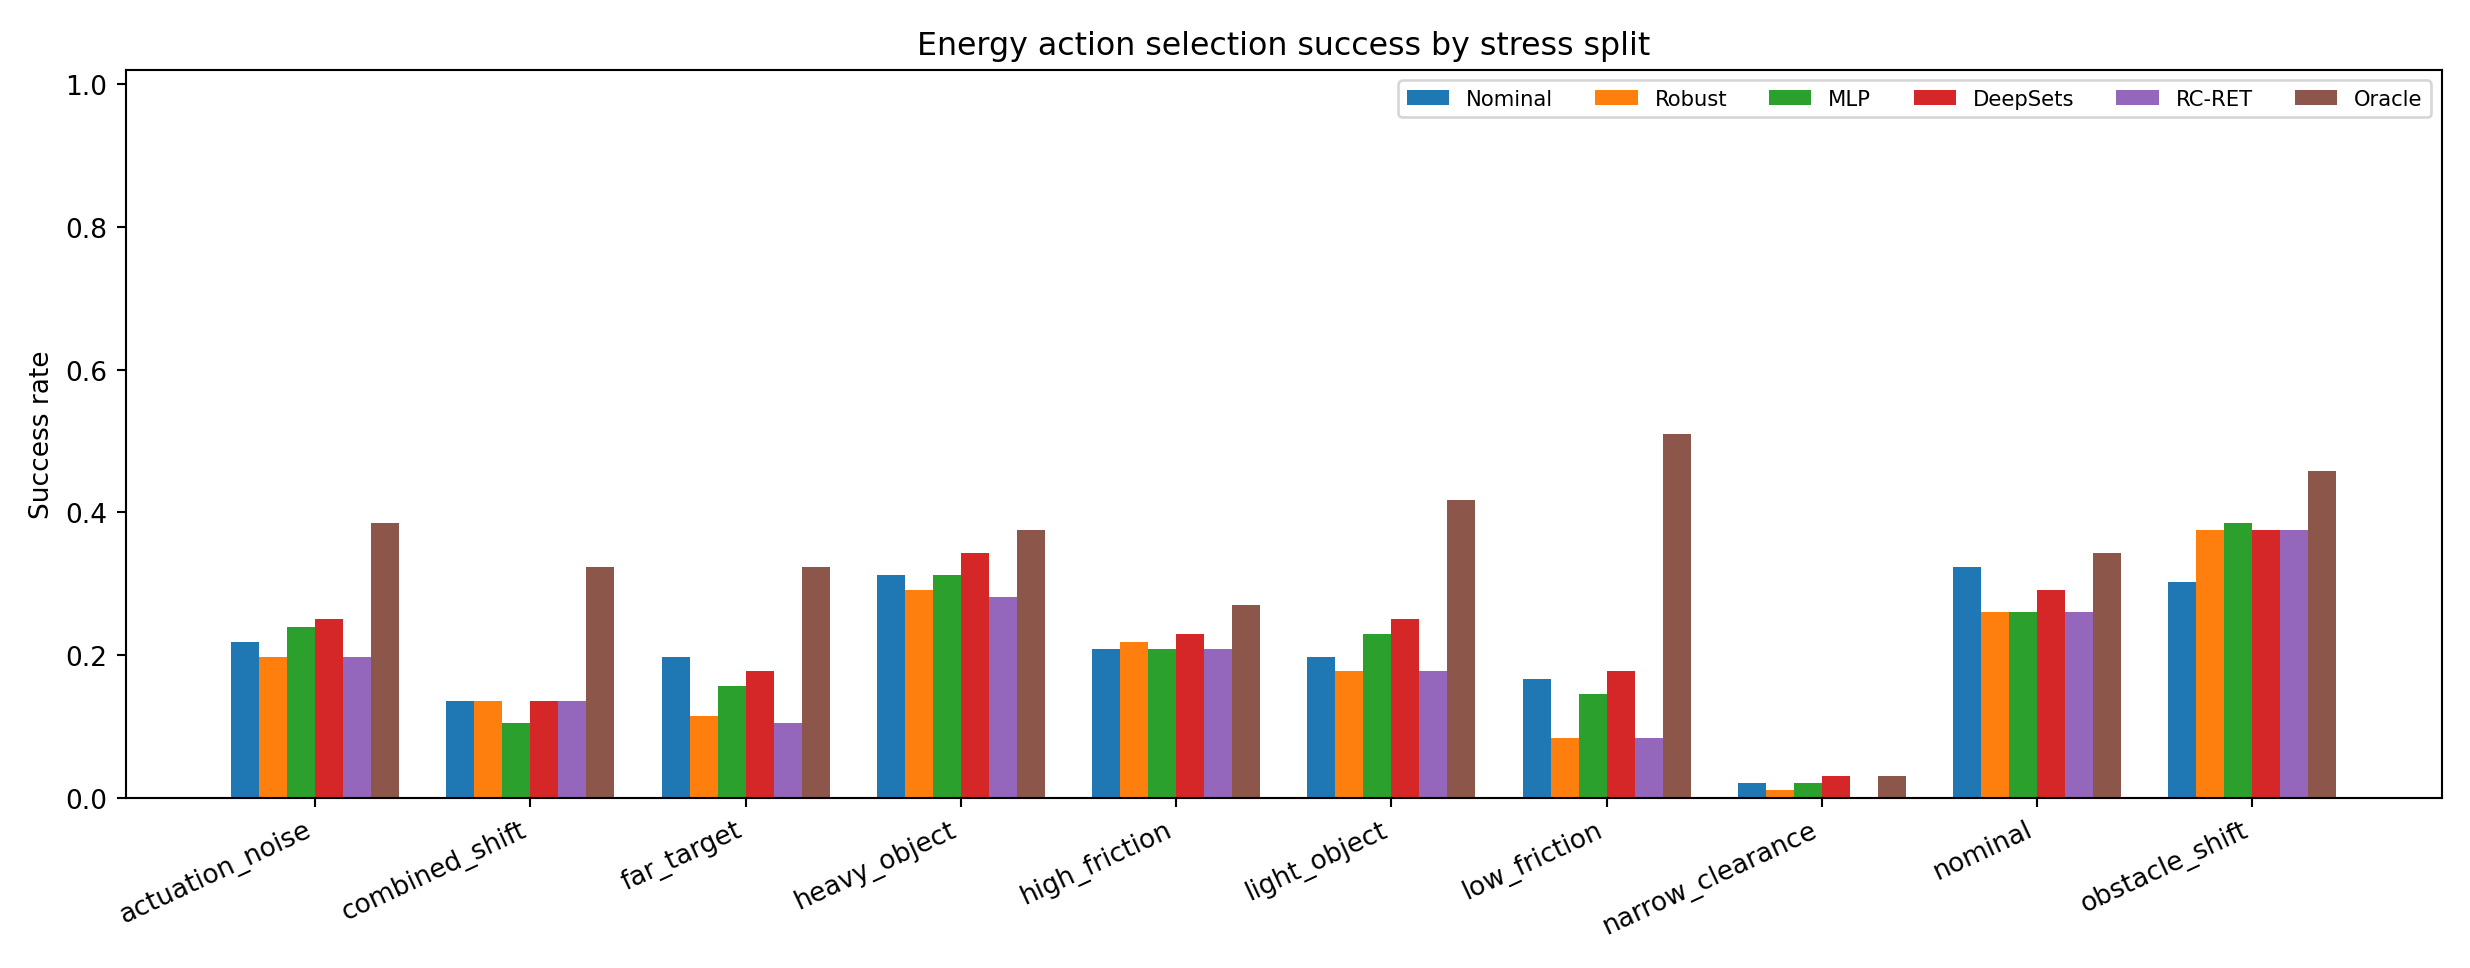
\includegraphics[width=\linewidth]{../figures/energy_success_by_split.png}
\caption{Frozen v5 success rates across stress splits.  \method{} is competitive with robust/CVaR branch scoring on several splits but does not separate from MLP, Deep Sets, or the oracle.}
\label{fig:success}
\end{figure}

\begin{figure}[t]
\centering
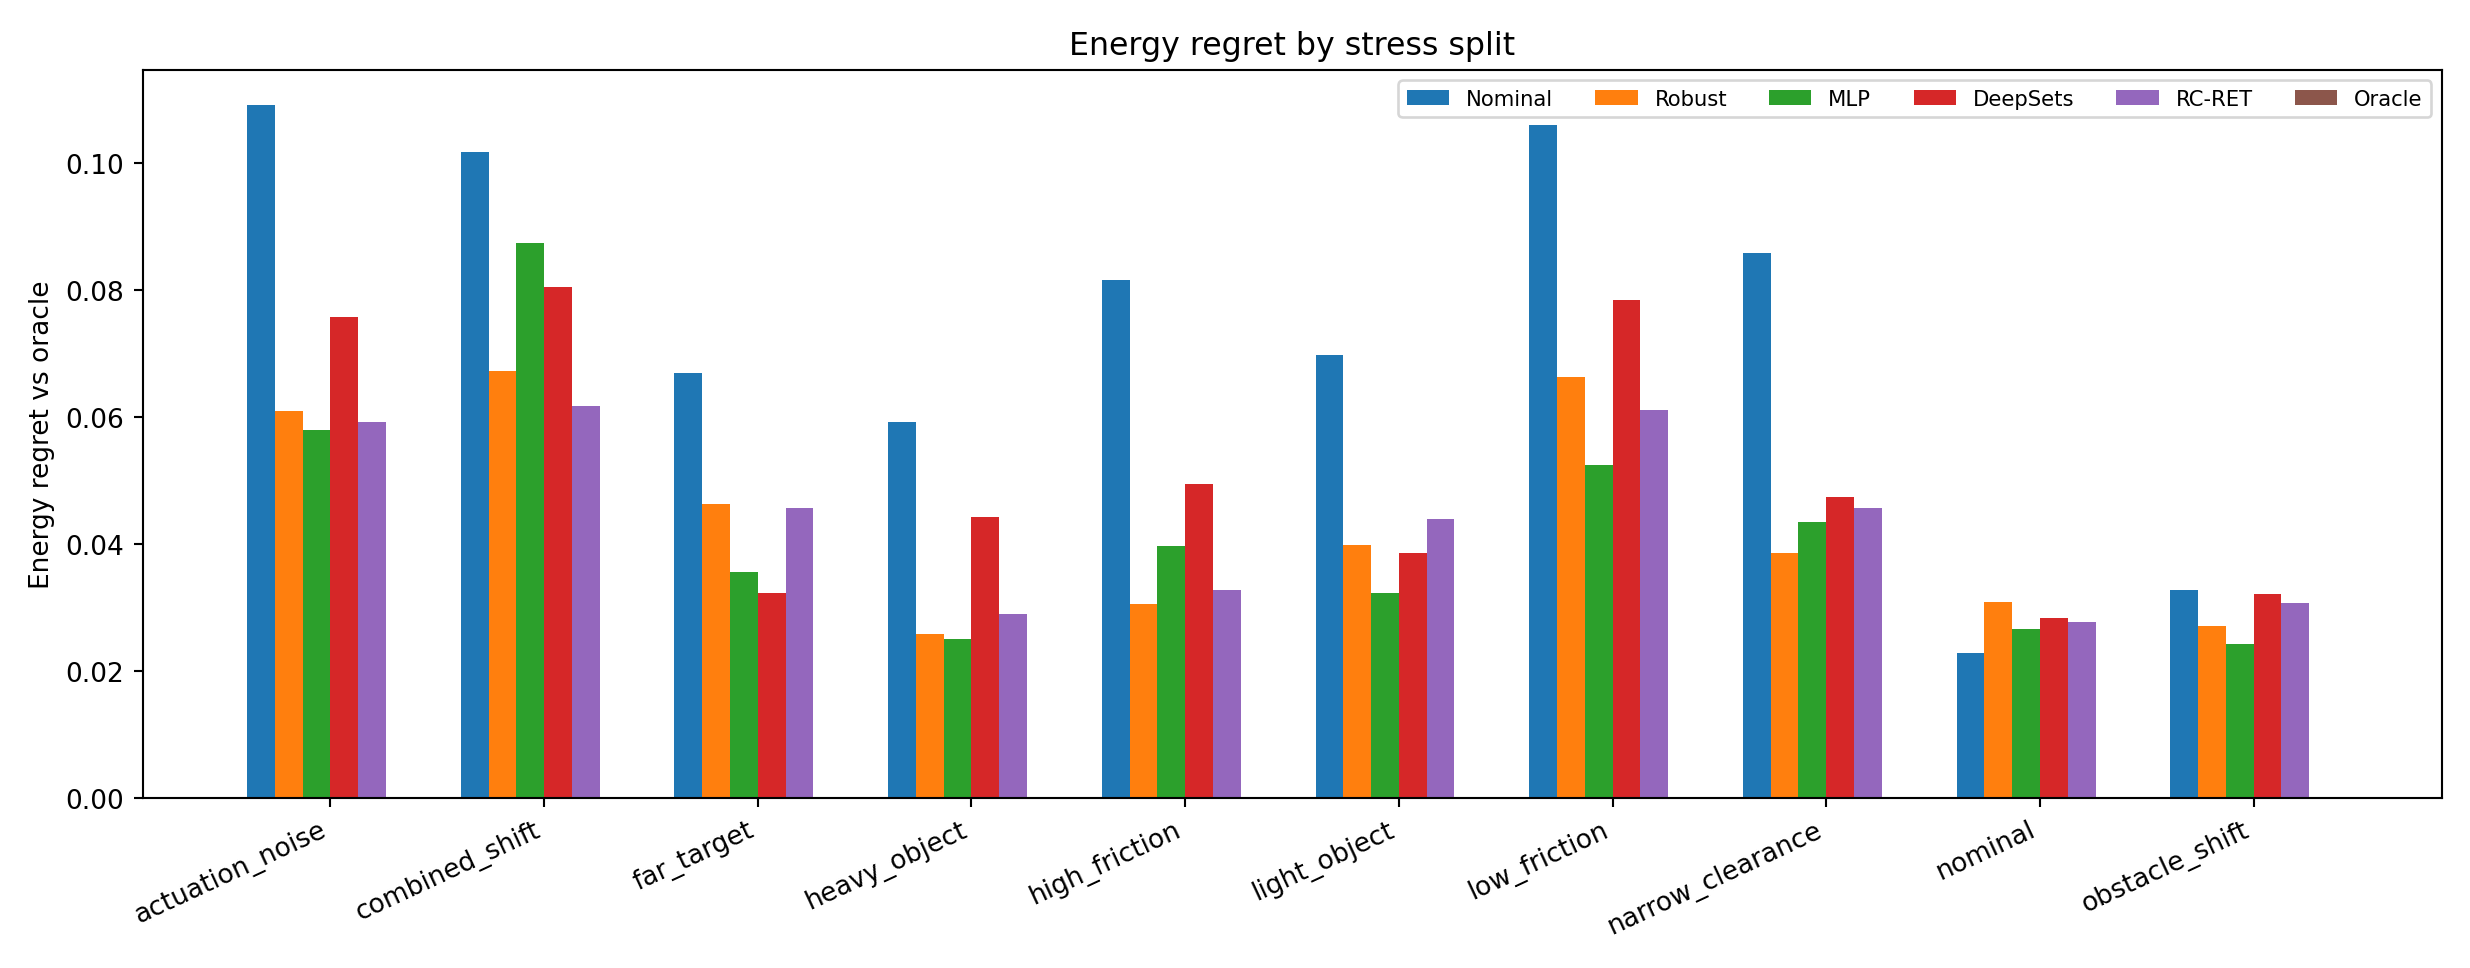
\includegraphics[width=\linewidth]{../figures/energy_regret_by_split.png}
\caption{Energy regret against the true MuJoCo rollout oracle.  Lower is better.  \method{} remains close to robust branch scoring, but this is not enough for an ICLR-main positive claim.}
\label{fig:regret}
\end{figure}

\begin{figure}[t]
\centering
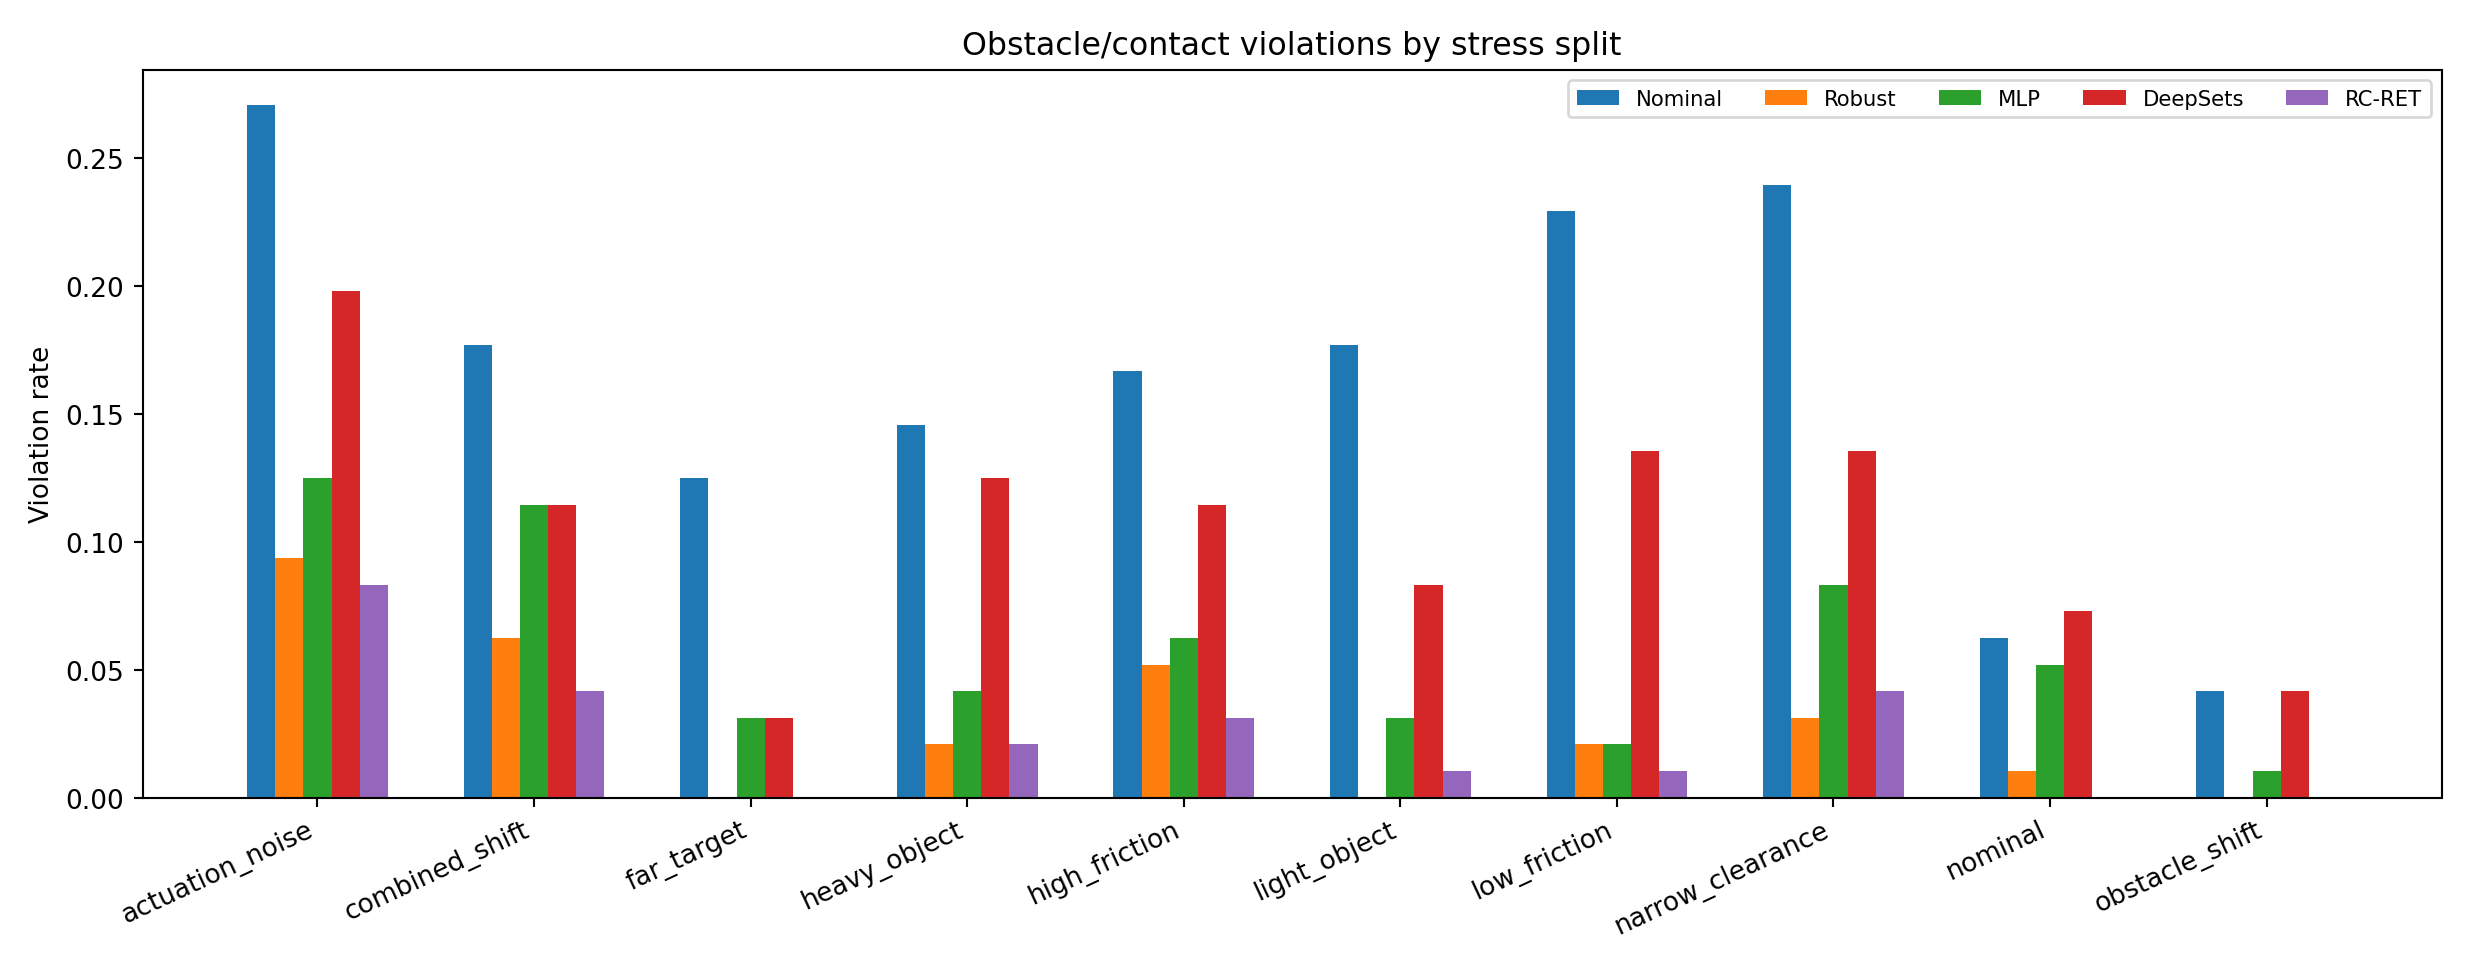
\includegraphics[width=\linewidth]{../figures/energy_violation_by_split.png}
\caption{Obstacle/contact violation rate.  The shield reduces several learned-model violation modes, but safety gains alone do not compensate for the missing success advantage.}
\label{fig:violation}
\end{figure}

\begin{figure}[t]
\centering
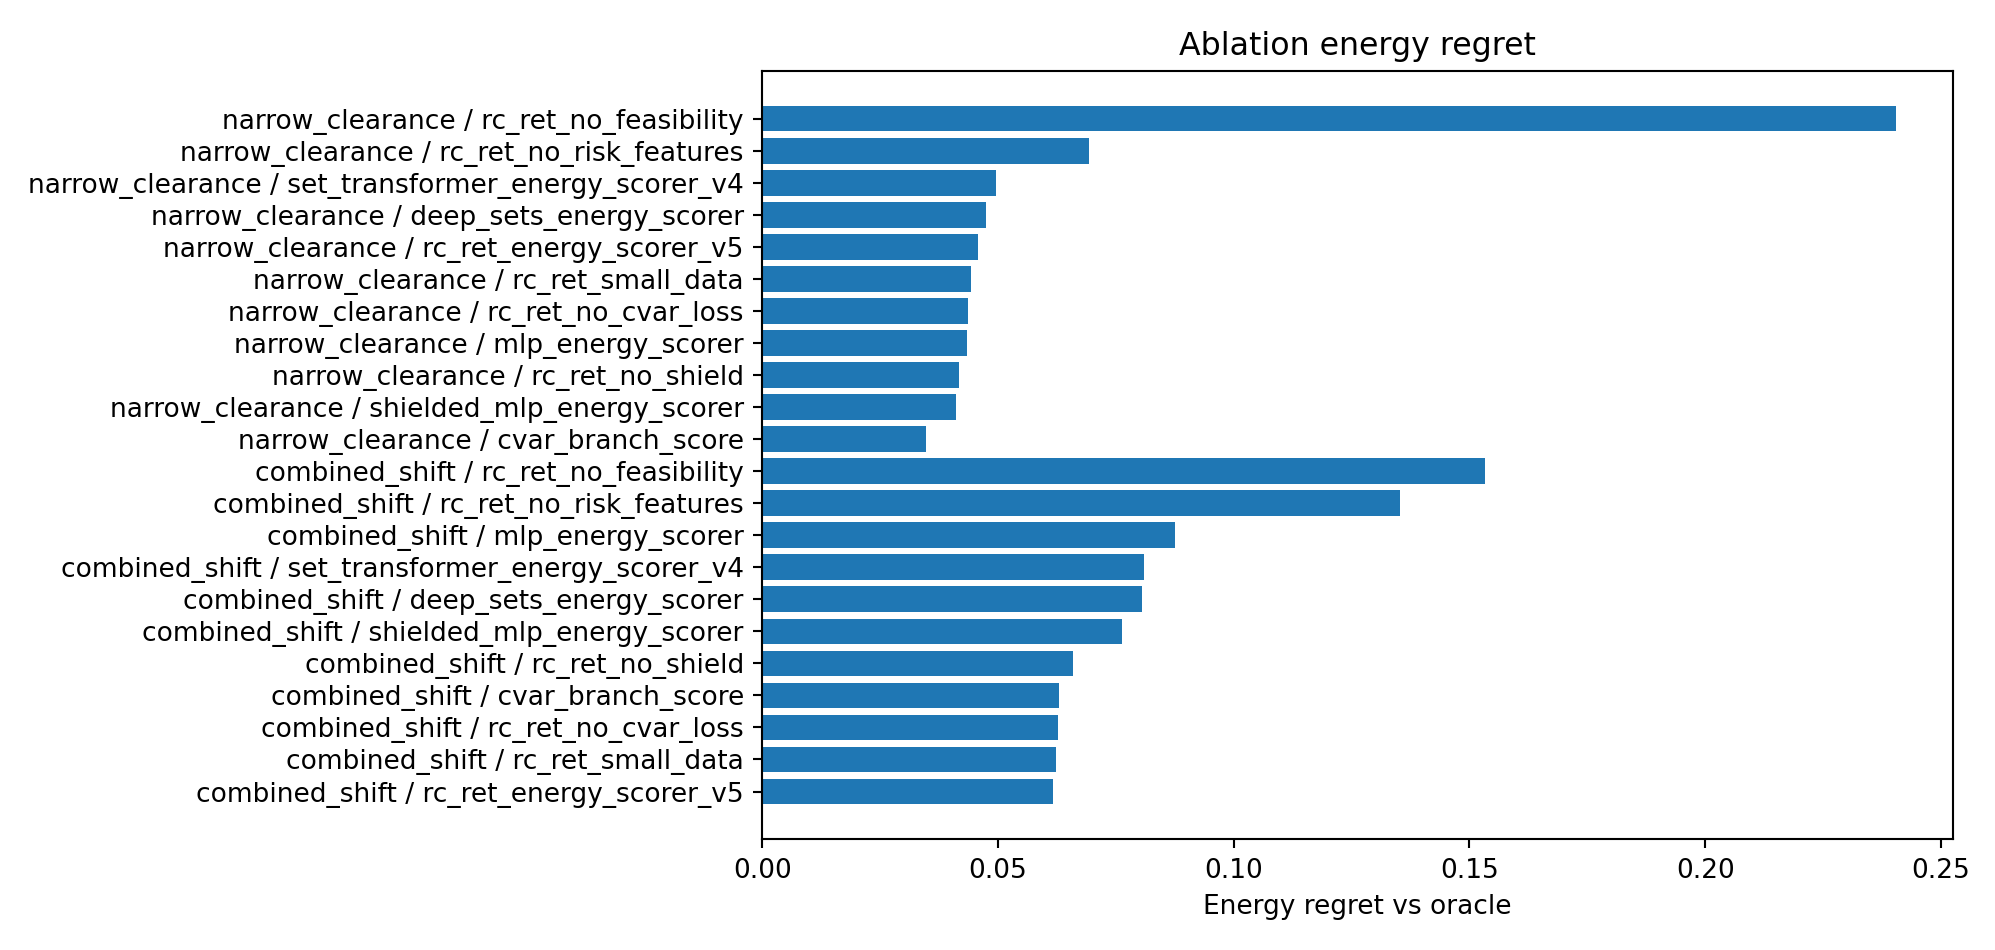
\includegraphics[width=0.90\linewidth]{../figures/energy_ablation_regret.png}
\caption{Ablation regret on combined-shift and narrow-clearance stress.  Removing feasibility causes severe violations; removing risk features hurts regret, but the full method still does not dominate all strong baselines.}
\label{fig:ablation}
\end{figure}

\subsection{Main Finding}

The final result is mixed.  \method{} has reasonable regret and low violation rates, but its success rate does not beat strong baselines.  Aggregate paired deltas show that \method{} loses success against nominal MPC by $-0.0260$, MLP by $-0.0240$, Deep Sets by $-0.0437$, and the old v4 transformer by $-0.0427$.  It is close to robust MPC ($-0.0042$) and branch-CVaR scoring ($+0.0010$), but closeness is not a main-conference contribution.

The best evidence for \method{} is safety.  Against MLP, the aggregate violation delta is $-0.0333$; against Deep Sets, $-0.0813$; against nominal MPC, $-0.1396$.  This supports the claim that feasibility calibration matters.  It does not support the stronger claim that a relational energy transformer is the best action selector.

\subsection{Split-Level Behavior}

On nominal scenes, \method{} reaches $26.0\%$ success, matching MLP and robust/CVaR branch scoring while maintaining zero violations.  On obstacle shift, it reaches $37.5\%$ success with zero violations, but MLP and shielded MLP are also strong.  On combined shift, \method{} ties branch-CVaR and Deep Sets at $13.5\%$ success and has lower regret than MLP, but the oracle remains far higher at $32.3\%$.

The narrow-clearance split is the strongest negative case.  \method{} records $0.0\%$ success and $4.17\%$ violations, while the oracle records $3.12\%$ success.  This is not a numerical accident.  The split deliberately generates cases where the finite primitive library is too coarse for the available clearance.  A better model over the same candidates cannot manufacture an absent primitive.

\subsection{Ablations}

The ablations support some but not all of the method design.  Removing feasibility is catastrophic: violation rises to $44.8\%$ on combined shift and $93.8\%$ on narrow clearance.  Removing risk features drops combined-shift success to zero and raises regret.  Removing the shield increases some violations.  These are real mechanisms.

However, the ablations do not isolate attention as decisively necessary.  Deep Sets and MLP remain competitive on several splits.  Small-data \method{} is close to full \method{} in combined shift.  This means the paper cannot claim that transformer attention is the decisive ingredient.

\section{Failure Analysis}

\paragraph{Finite candidate failure.}
The candidate library is richer than v4, but it is still discrete.  Narrow-clearance scenes sometimes require a carefully curved or multi-stage primitive.  A finite one-stage library may contain no safe high-progress action.  The regret decomposition predicts exactly this failure.

\paragraph{Hidden latent ambiguity.}
Mass and friction are not observed directly.  Two latent parameter settings can produce identical candidate features but reverse the best action.  Without additional sensing or online adaptation, any deterministic selector must fail in at least one of those worlds.

\paragraph{Shield conservatism.}
The shield protects modeled branch clearances, but it can select a lower-progress action.  Shield activation is reported because hiding it would make the method look cleaner than it is.

\paragraph{Strong baselines are genuinely strong.}
Robust MPC and branch-CVaR scoring use exact branch rollouts and are hard to beat when the branch set is well aligned with test shifts.  This is a feature of the benchmark, not a problem.  A submission-ready learned method must beat this bar honestly.

\section{Related Work}

\paragraph{Energy-based action selection.}
Energy-based learning provides a natural language for ranking actions by scalar compatibility or cost \citep{lecun2006tutorial}.  Implicit behavioral cloning showed that energy-based policies can represent multimodal action distributions without committing to a simple Gaussian decoder \citep{florence2022implicit}.  Our setting differs because the action set is generated explicitly and every candidate can be rolled out in simulation; the question is whether learned set calibration improves selection under contact shifts.

\paragraph{Set models and transformers.}
Deep Sets formalized permutation-invariant/equivariant processing for unordered sets \citep{zaheer2017deep}.  Set Transformer added attention-based interactions among set elements \citep{lee2019set}, building on the transformer architecture \citep{vaswani2017attention}.  The present paper treats attention as a hypothesis, not an assumption.  Deep Sets is included because permutation equivariance alone is not enough to justify a transformer.

\paragraph{Robot policy learning.}
Diffusion Policy and Action Chunking Transformers show the strength of expressive action-distribution models for robot control \citep{chi2023diffusion,zhao2023learning}.  Those methods typically learn policies from large demonstration datasets.  Our benchmark is narrower: a finite action library is generated online, and the selector ranks candidates using rollout-labeled energy and branch risk.

\paragraph{Model-based and robust control.}
MPPI and PETS demonstrate the value of sampling and uncertainty in model-based control \citep{williams2017mppi,chua2018pets}.  Robust MPC emphasizes stability and constraint satisfaction under uncertainty \citep{mayne2000constrained}.  These ideas motivate the robust and CVaR baselines.  The final result confirms that robust control is not an easy baseline to beat in contact-rich action selection.

\paragraph{Simulation.}
MuJoCo is widely used for model-based control and contact-rich robot simulation \citep{todorov2012mujoco}.  The paper uses MuJoCo for both training labels and evaluation rollouts.  This is better than synthetic evidence, but it is not hardware validation.

\section{Limitations}

This is still a custom MuJoCo benchmark, not a public manipulation benchmark and not hardware.  The action library is finite and manually parameterized.  The branch set is small.  The models operate on compact tabular features, not visual inputs.  The theory gives limited guarantees under modeled branches and calibrated errors; it does not certify real-world safety.  Most importantly, the core positive claim fails the frozen gate.  \method{} is useful, but not yet a submission-ready main-conference contribution.

\section{Conclusion}

This paper turns a weak energy-transformer idea into a rigorous strong-revise evidence package.  The method is more principled, the experiments are larger, the baselines are stronger, the citations are real, and the negative result is clearer.  The outcome is not the glamorous one: \method{} does not deserve an ICLR-main-ready claim.  That is precisely why the study is useful.  It shows what an action-set energy method must still solve: richer primitive generation, better online latent inference, stronger public/hardware validation, and a mechanism that beats Deep Sets, MLPs, and robust MPC without paying for safety with lost success.

\clearpage
\appendix

\section{Reproducibility Checklist}

The repository contains the full runner, frozen protocol, raw CSVs, summary CSVs, figures, and PDF build scripts.  The frozen command is recorded in `docs/paper62\_protocol\_freeze\_20260619.md`.  The final decision summary is recorded in `docs/paper62\_final\_v5\_evidence\_summary.md`.  The build script renders tables, writes the evidence summary, compiles LaTeX with BibTeX, and copies the final PDF only to Downloads.

\paragraph{Hardware.}
The run was CPU-only.  Torch threads were capped at 4.  The runner stores compact NumPy arrays and CSVs and avoids image tensors or large replay buffers.

\paragraph{Rows.}
The main raw CSV contains 11,520 rows.  The ablation raw CSV contains 2,112 rows.  The metric CSV contains 120 rows.  The ablation summary contains 22 rows.  The pairwise table contains 99 rows.

\paragraph{No cherry-picking.}
Development smoke tests were used only before the protocol freeze.  After `paper62\_protocol\_freeze\_20260619.md`, the final run reported every predefined split, method, seed, and ablation.

\section{Algorithm Details}

\paragraph{Training data generation.}
For each training action set, the script samples a split, state, target, obstacle, mass, and friction.  For every candidate action it performs MuJoCo branch rollouts, true-parameter rollout, and label construction.  The resulting tensor has shape $480 \times 63 \times 29$ after standardization.

\paragraph{Model training.}
The MLP is trained on flattened candidate rows.  Deep Sets, v4 transformer, and \method{} are trained on full candidate sets.  \method{} has separate energy and violation heads.  All models use AdamW, small hidden widths, and CPU tensor operations.

\paragraph{Evaluation.}
For each test episode, candidate features and true outcomes are computed once and shared across methods.  This ensures paired comparisons are meaningful.  Learned models score standardized features.  MPC-style and branch-score baselines use the same branch summaries.

\section{Proof Details}

The equivariance proposition assumes no positional encodings.  Candidate order is arbitrary; adding position embeddings would break the symmetry unless the embeddings were themselves permutation-consistent.  The implementation uses no positional embeddings.  Rank features are values attached to candidate tokens, not order indices, so they do not break equivariance.

The regret decomposition is intentionally loose.  It is designed to identify failure modes rather than produce a tight numerical bound.  A tighter analysis would require assumptions about Lipschitz continuity of the simulator with respect to contact parameters and primitive geometry.  Those assumptions are not safe in contact-rich manipulation, where small clearance changes can flip collision outcomes.

The safety lemma is also local to the modeled branch set.  It should not be read as a hardware safety certificate.  In real deployment, a shield would need calibrated perception, online contact estimation, actuator limits, and runtime monitoring.

\section{Split Cards}

\paragraph{Nominal.}
Mass and friction vary near the training center.  Obstacles are moderately offset from the direct path.  This split tests whether the method harms easy cases.

\paragraph{Low friction.}
Friction values are lower than nominal, making pushes travel farther and making aggressive primitives risky.  The oracle gap is large because hidden friction matters.

\paragraph{High friction.}
Friction values are higher than nominal, making progress harder and increasing the value of longer pushes.  Robust and branch-risk baselines are strong here.

\paragraph{Light object.}
Mass is lower and actuation noise is present.  Some actions overshoot.  The finite action library must trade progress against control.

\paragraph{Heavy object.}
Mass is higher.  Low-effort primitives often underperform.  Learned models can overfit to nominal progress features.

\paragraph{Obstacle shift.}
Obstacle location varies more than in nominal scenes.  Feasibility features and shields matter.

\paragraph{Narrow clearance.}
The obstacle lies close to the direct path.  Many scenes have no safe high-progress primitive in the finite library.  This is the strongest negative split.

\paragraph{Actuation noise.}
The action path is perturbed during evaluation.  Deterministic branch planning becomes less reliable.

\paragraph{Far target.}
Targets are farther away, increasing the cost of conservative pushes.  Candidate discretization becomes more visible.

\paragraph{Combined shift.}
Mass, friction, obstacle placement, target distance, and actuation noise shift simultaneously.  This split is the main stress gate.

\section{Hyperparameters}

\begin{table}[h]
\centering
\caption{Frozen hyperparameters.}
\label{tab:hyperparams}
\small
\begin{tabular}{lr}
\toprule
Quantity & Value \\
\midrule
Training action sets & 480 \\
Epochs & 24 \\
Seeds & 8 \\
Episodes per split/seed & 12 \\
Candidate actions & 63 \\
Torch threads & 4 \\
Energy effort coefficient & 0.03 \\
Violation penalty & 0.32 \\
Success radius & 0.075 \\
Contact margin & puck radius + obstacle radius + 0.006 \\
Shield buffer & 0.002 \\
Transformer hidden width & 64 \\
Transformer layers & 2 \\
Attention heads & 4 \\
\bottomrule
\end{tabular}
\end{table}

\section{Additional Interpretation of Generated Tables}

Table~\ref{tab:v5-success} is the most important table for acceptance readiness.  It shows that \method{} is not a success-rate winner.  Table~\ref{tab:v5-regret} is more favorable: \method{} is often close to robust/CVaR scoring and sometimes beats MLP on regret.  Table~\ref{tab:v5-pairwise} resolves the conflict: the aggregate evidence is not strong enough to claim a main-conference positive result.  Table~\ref{tab:v5-ablation} explains why the paper is still worth preserving: feasibility and risk features matter, even though attention is not isolated as the decisive mechanism.

\clearpage
\section{Full Frozen Metric Tables}

This appendix includes the complete split-level summary used for the terminal decision.  These tables are intentionally repetitive: hostile review often turns on a single split or baseline that a short main paper hides.  Each table is generated directly from the frozen CSVs by `scripts/render\_latex\_tables.py`.

% Auto-generated detailed metric tables
\begin{table}[p]
\centering
\caption{Detailed frozen metrics for nominal.}
\label{tab:detail-nominal}
\small
\begin{tabular}{lrrrrr}
\toprule
Method & Success & Regret & Distance & Violation & Shield \\
\midrule
cvar\_branch\_score & 26.0 & 0.029 & 0.127 & 0.0 & 5.2 \\
deep\_sets\_energy\_scorer & 29.2 & 0.028 & 0.102 & 7.3 & 0.0 \\
geometric\_greedy & 0.0 & 0.240 & 0.222 & 35.4 & 0.0 \\
mlp\_energy\_scorer & 26.0 & 0.027 & 0.107 & 5.2 & 0.0 \\
nominal\_rollout\_mpc & 32.3 & 0.023 & 0.099 & 6.2 & 0.0 \\
oracle\_mujoco\_rollout\_selector & 34.4 & 0.000 & 0.095 & 0.0 & 0.0 \\
random\_candidate & 0.0 & 0.303 & 0.265 & 41.7 & 0.0 \\
rc\_ret\_energy\_scorer\_v5 & 26.0 & 0.028 & 0.126 & 0.0 & 6.2 \\
rc\_ret\_no\_shield & 27.1 & 0.028 & 0.122 & 1.0 & 0.0 \\
robust\_worst\_case\_mpc & 26.0 & 0.031 & 0.126 & 1.0 & 0.0 \\
set\_transformer\_energy\_scorer\_v4 & 27.1 & 0.033 & 0.107 & 7.3 & 0.0 \\
shielded\_mlp\_energy\_scorer & 22.9 & 0.023 & 0.119 & 0.0 & 17.7 \\
\bottomrule
\end{tabular}
\end{table}

\begin{table}[p]
\centering
\caption{Detailed frozen metrics for low\_friction.}
\label{tab:detail-low-friction}
\small
\begin{tabular}{lrrrrr}
\toprule
Method & Success & Regret & Distance & Violation & Shield \\
\midrule
cvar\_branch\_score & 8.3 & 0.068 & 0.152 & 1.0 & 9.4 \\
deep\_sets\_energy\_scorer & 17.7 & 0.078 & 0.122 & 13.5 & 0.0 \\
geometric\_greedy & 0.0 & 0.279 & 0.194 & 53.1 & 0.0 \\
mlp\_energy\_scorer & 14.6 & 0.052 & 0.133 & 2.1 & 0.0 \\
nominal\_rollout\_mpc & 16.7 & 0.106 & 0.118 & 22.9 & 0.0 \\
oracle\_mujoco\_rollout\_selector & 51.0 & 0.000 & 0.085 & 0.0 & 0.0 \\
random\_candidate & 2.1 & 0.317 & 0.288 & 35.4 & 0.0 \\
rc\_ret\_energy\_scorer\_v5 & 8.3 & 0.061 & 0.145 & 1.0 & 9.4 \\
rc\_ret\_no\_shield & 8.3 & 0.061 & 0.142 & 2.1 & 0.0 \\
robust\_worst\_case\_mpc & 8.3 & 0.066 & 0.147 & 2.1 & 0.0 \\
set\_transformer\_energy\_scorer\_v4 & 17.7 & 0.057 & 0.127 & 5.2 & 0.0 \\
shielded\_mlp\_energy\_scorer & 11.5 & 0.059 & 0.141 & 1.0 & 15.6 \\
\bottomrule
\end{tabular}
\end{table}

\begin{table}[p]
\centering
\caption{Detailed frozen metrics for high\_friction.}
\label{tab:detail-high-friction}
\small
\begin{tabular}{lrrrrr}
\toprule
Method & Success & Regret & Distance & Violation & Shield \\
\midrule
cvar\_branch\_score & 20.8 & 0.028 & 0.130 & 3.1 & 6.2 \\
deep\_sets\_energy\_scorer & 22.9 & 0.050 & 0.124 & 11.5 & 0.0 \\
geometric\_greedy & 0.0 & 0.199 & 0.246 & 19.8 & 0.0 \\
mlp\_energy\_scorer & 20.8 & 0.040 & 0.131 & 6.2 & 0.0 \\
nominal\_rollout\_mpc & 20.8 & 0.082 & 0.138 & 16.7 & 0.0 \\
oracle\_mujoco\_rollout\_selector & 27.1 & 0.000 & 0.112 & 0.0 & 0.0 \\
random\_candidate & 1.0 & 0.283 & 0.273 & 37.5 & 0.0 \\
rc\_ret\_energy\_scorer\_v5 & 20.8 & 0.033 & 0.135 & 3.1 & 6.2 \\
rc\_ret\_no\_shield & 21.9 & 0.037 & 0.132 & 5.2 & 0.0 \\
robust\_worst\_case\_mpc & 21.9 & 0.031 & 0.126 & 5.2 & 0.0 \\
set\_transformer\_energy\_scorer\_v4 & 24.0 & 0.045 & 0.123 & 10.4 & 0.0 \\
shielded\_mlp\_energy\_scorer & 19.8 & 0.036 & 0.137 & 3.1 & 9.4 \\
\bottomrule
\end{tabular}
\end{table}

\begin{table}[p]
\centering
\caption{Detailed frozen metrics for light\_object.}
\label{tab:detail-light-object}
\small
\begin{tabular}{lrrrrr}
\toprule
Method & Success & Regret & Distance & Violation & Shield \\
\midrule
cvar\_branch\_score & 17.7 & 0.040 & 0.137 & 0.0 & 3.1 \\
deep\_sets\_energy\_scorer & 25.0 & 0.039 & 0.108 & 8.3 & 0.0 \\
geometric\_greedy & 1.0 & 0.281 & 0.213 & 51.0 & 0.0 \\
mlp\_energy\_scorer & 22.9 & 0.032 & 0.119 & 3.1 & 0.0 \\
nominal\_rollout\_mpc & 19.8 & 0.070 & 0.108 & 17.7 & 0.0 \\
oracle\_mujoco\_rollout\_selector & 41.7 & 0.000 & 0.095 & 0.0 & 0.0 \\
random\_candidate & 1.0 & 0.306 & 0.277 & 38.5 & 0.0 \\
rc\_ret\_energy\_scorer\_v5 & 17.7 & 0.044 & 0.138 & 1.0 & 8.3 \\
rc\_ret\_no\_shield & 17.7 & 0.040 & 0.134 & 1.0 & 0.0 \\
robust\_worst\_case\_mpc & 17.7 & 0.040 & 0.137 & 0.0 & 0.0 \\
set\_transformer\_energy\_scorer\_v4 & 26.0 & 0.033 & 0.114 & 5.2 & 0.0 \\
shielded\_mlp\_energy\_scorer & 20.8 & 0.031 & 0.124 & 1.0 & 10.4 \\
\bottomrule
\end{tabular}
\end{table}

\begin{table}[p]
\centering
\caption{Detailed frozen metrics for heavy\_object.}
\label{tab:detail-heavy-object}
\small
\begin{tabular}{lrrrrr}
\toprule
Method & Success & Regret & Distance & Violation & Shield \\
\midrule
cvar\_branch\_score & 28.1 & 0.023 & 0.116 & 1.0 & 5.2 \\
deep\_sets\_energy\_scorer & 34.4 & 0.044 & 0.101 & 12.5 & 0.0 \\
geometric\_greedy & 0.0 & 0.239 & 0.205 & 40.6 & 0.0 \\
mlp\_energy\_scorer & 31.2 & 0.025 & 0.109 & 4.2 & 0.0 \\
nominal\_rollout\_mpc & 31.2 & 0.059 & 0.108 & 14.6 & 0.0 \\
oracle\_mujoco\_rollout\_selector & 37.5 & 0.000 & 0.096 & 0.0 & 0.0 \\
random\_candidate & 0.0 & 0.308 & 0.236 & 52.1 & 0.0 \\
rc\_ret\_energy\_scorer\_v5 & 28.1 & 0.029 & 0.119 & 2.1 & 5.2 \\
rc\_ret\_no\_shield & 29.2 & 0.030 & 0.117 & 3.1 & 0.0 \\
robust\_worst\_case\_mpc & 29.2 & 0.026 & 0.116 & 2.1 & 0.0 \\
set\_transformer\_energy\_scorer\_v4 & 33.3 & 0.044 & 0.104 & 11.5 & 0.0 \\
shielded\_mlp\_energy\_scorer & 28.1 & 0.020 & 0.116 & 0.0 & 10.4 \\
\bottomrule
\end{tabular}
\end{table}

\begin{table}[p]
\centering
\caption{Detailed frozen metrics for obstacle\_shift.}
\label{tab:detail-obstacle-shift}
\small
\begin{tabular}{lrrrrr}
\toprule
Method & Success & Regret & Distance & Violation & Shield \\
\midrule
cvar\_branch\_score & 37.5 & 0.029 & 0.121 & 0.0 & 3.1 \\
deep\_sets\_energy\_scorer & 37.5 & 0.032 & 0.110 & 4.2 & 0.0 \\
geometric\_greedy & 0.0 & 0.230 & 0.223 & 30.2 & 0.0 \\
mlp\_energy\_scorer & 38.5 & 0.024 & 0.112 & 1.0 & 0.0 \\
nominal\_rollout\_mpc & 30.2 & 0.033 & 0.109 & 4.2 & 0.0 \\
oracle\_mujoco\_rollout\_selector & 45.8 & 0.000 & 0.090 & 0.0 & 0.0 \\
random\_candidate & 1.0 & 0.299 & 0.262 & 39.6 & 0.0 \\
rc\_ret\_energy\_scorer\_v5 & 37.5 & 0.031 & 0.123 & 0.0 & 4.2 \\
rc\_ret\_no\_shield & 37.5 & 0.029 & 0.121 & 0.0 & 0.0 \\
robust\_worst\_case\_mpc & 37.5 & 0.027 & 0.119 & 0.0 & 0.0 \\
set\_transformer\_energy\_scorer\_v4 & 37.5 & 0.023 & 0.107 & 2.1 & 0.0 \\
shielded\_mlp\_energy\_scorer & 38.5 & 0.024 & 0.115 & 0.0 & 8.3 \\
\bottomrule
\end{tabular}
\end{table}

\begin{table}[p]
\centering
\caption{Detailed frozen metrics for narrow\_clearance.}
\label{tab:detail-narrow-clearance}
\small
\begin{tabular}{lrrrrr}
\toprule
Method & Success & Regret & Distance & Violation & Shield \\
\midrule
cvar\_branch\_score & 0.0 & 0.035 & 0.197 & 3.1 & 7.3 \\
deep\_sets\_energy\_scorer & 3.1 & 0.047 & 0.176 & 13.5 & 0.0 \\
geometric\_greedy & 0.0 & 0.262 & 0.247 & 58.3 & 0.0 \\
mlp\_energy\_scorer & 2.1 & 0.043 & 0.189 & 8.3 & 0.0 \\
nominal\_rollout\_mpc & 2.1 & 0.086 & 0.179 & 24.0 & 0.0 \\
oracle\_mujoco\_rollout\_selector & 3.1 & 0.000 & 0.171 & 0.0 & 0.0 \\
random\_candidate & 0.0 & 0.276 & 0.293 & 47.9 & 0.0 \\
rc\_ret\_energy\_scorer\_v5 & 0.0 & 0.046 & 0.205 & 4.2 & 6.2 \\
rc\_ret\_no\_shield & 1.0 & 0.042 & 0.201 & 4.2 & 0.0 \\
robust\_worst\_case\_mpc & 1.0 & 0.039 & 0.201 & 3.1 & 0.0 \\
set\_transformer\_energy\_scorer\_v4 & 3.1 & 0.050 & 0.176 & 14.6 & 0.0 \\
shielded\_mlp\_energy\_scorer & 0.0 & 0.041 & 0.196 & 5.2 & 13.5 \\
\bottomrule
\end{tabular}
\end{table}

\begin{table}[p]
\centering
\caption{Detailed frozen metrics for actuation\_noise.}
\label{tab:detail-actuation-noise}
\small
\begin{tabular}{lrrrrr}
\toprule
Method & Success & Regret & Distance & Violation & Shield \\
\midrule
cvar\_branch\_score & 18.8 & 0.061 & 0.138 & 8.3 & 6.2 \\
deep\_sets\_energy\_scorer & 25.0 & 0.076 & 0.116 & 19.8 & 0.0 \\
geometric\_greedy & 0.0 & 0.252 & 0.227 & 39.6 & 0.0 \\
mlp\_energy\_scorer & 24.0 & 0.058 & 0.121 & 12.5 & 0.0 \\
nominal\_rollout\_mpc & 21.9 & 0.109 & 0.124 & 27.1 & 0.0 \\
oracle\_mujoco\_rollout\_selector & 38.5 & 0.000 & 0.101 & 0.0 & 0.0 \\
random\_candidate & 1.0 & 0.312 & 0.273 & 43.8 & 0.0 \\
rc\_ret\_energy\_scorer\_v5 & 19.8 & 0.059 & 0.136 & 8.3 & 9.4 \\
rc\_ret\_no\_shield & 20.8 & 0.062 & 0.132 & 10.4 & 0.0 \\
robust\_worst\_case\_mpc & 19.8 & 0.061 & 0.135 & 9.4 & 0.0 \\
set\_transformer\_energy\_scorer\_v4 & 26.0 & 0.067 & 0.114 & 17.7 & 0.0 \\
shielded\_mlp\_energy\_scorer & 20.8 & 0.062 & 0.135 & 9.4 & 13.5 \\
\bottomrule
\end{tabular}
\end{table}

\begin{table}[p]
\centering
\caption{Detailed frozen metrics for far\_target.}
\label{tab:detail-far-target}
\small
\begin{tabular}{lrrrrr}
\toprule
Method & Success & Regret & Distance & Violation & Shield \\
\midrule
cvar\_branch\_score & 10.4 & 0.050 & 0.155 & 1.0 & 1.0 \\
deep\_sets\_energy\_scorer & 17.7 & 0.032 & 0.130 & 3.1 & 0.0 \\
geometric\_greedy & 0.0 & 0.309 & 0.294 & 37.5 & 0.0 \\
mlp\_energy\_scorer & 15.6 & 0.035 & 0.133 & 3.1 & 0.0 \\
nominal\_rollout\_mpc & 19.8 & 0.067 & 0.133 & 12.5 & 0.0 \\
oracle\_mujoco\_rollout\_selector & 32.3 & 0.000 & 0.107 & 0.0 & 0.0 \\
random\_candidate & 1.0 & 0.392 & 0.383 & 35.4 & 0.0 \\
rc\_ret\_energy\_scorer\_v5 & 10.4 & 0.046 & 0.155 & 0.0 & 2.1 \\
rc\_ret\_no\_shield & 12.5 & 0.042 & 0.151 & 0.0 & 0.0 \\
robust\_worst\_case\_mpc & 11.5 & 0.046 & 0.155 & 0.0 & 0.0 \\
set\_transformer\_energy\_scorer\_v4 & 17.7 & 0.039 & 0.127 & 6.2 & 0.0 \\
shielded\_mlp\_energy\_scorer & 11.5 & 0.046 & 0.143 & 3.1 & 14.6 \\
\bottomrule
\end{tabular}
\end{table}

\begin{table}[p]
\centering
\caption{Detailed frozen metrics for combined\_shift.}
\label{tab:detail-combined-shift}
\small
\begin{tabular}{lrrrrr}
\toprule
Method & Success & Regret & Distance & Violation & Shield \\
\midrule
cvar\_branch\_score & 13.5 & 0.063 & 0.166 & 4.2 & 6.2 \\
deep\_sets\_energy\_scorer & 13.5 & 0.080 & 0.159 & 11.5 & 0.0 \\
geometric\_greedy & 1.0 & 0.263 & 0.276 & 31.2 & 0.0 \\
mlp\_energy\_scorer & 10.4 & 0.087 & 0.166 & 11.5 & 0.0 \\
nominal\_rollout\_mpc & 13.5 & 0.102 & 0.159 & 17.7 & 0.0 \\
oracle\_mujoco\_rollout\_selector & 32.3 & 0.000 & 0.115 & 0.0 & 0.0 \\
random\_candidate & 0.0 & 0.325 & 0.341 & 30.2 & 0.0 \\
rc\_ret\_energy\_scorer\_v5 & 13.5 & 0.062 & 0.164 & 4.2 & 5.2 \\
rc\_ret\_no\_shield & 13.5 & 0.066 & 0.162 & 6.2 & 0.0 \\
robust\_worst\_case\_mpc & 13.5 & 0.067 & 0.164 & 6.2 & 0.0 \\
set\_transformer\_energy\_scorer\_v4 & 12.5 & 0.081 & 0.160 & 11.5 & 0.0 \\
shielded\_mlp\_energy\_scorer & 11.5 & 0.076 & 0.174 & 5.2 & 12.5 \\
\bottomrule
\end{tabular}
\end{table}


% Auto-generated detailed pairwise tables
\begin{table}[p]
\centering
\caption{Paired deltas for nominal. Positive success and regret-improvement favor RC-RET; negative violation deltas favor RC-RET.}
\label{tab:pair-nominal}
\small
\begin{tabular}{lrrrr}
\toprule
Baseline & Success $\Delta$ & Regret improv. & Distance improv. & Violation $\Delta$ \\
\midrule
nominal\_rollout\_mpc & -0.0625 & -0.0049 & -0.0267 & -0.0625 \\
robust\_worst\_case\_mpc & 0.0000 & 0.0031 & -0.0000 & -0.0104 \\
cvar\_branch\_score & 0.0000 & 0.0011 & 0.0012 & 0.0000 \\
mlp\_energy\_scorer & 0.0000 & -0.0011 & -0.0186 & -0.0521 \\
shielded\_mlp\_energy\_scorer & 0.0312 & -0.0051 & -0.0065 & 0.0000 \\
deep\_sets\_energy\_scorer & -0.0312 & 0.0006 & -0.0235 & -0.0729 \\
set\_transformer\_energy\_scorer\_v4 & -0.0104 & 0.0050 & -0.0188 & -0.0729 \\
oracle\_mujoco\_rollout\_selector & -0.0833 & -0.0277 & -0.0305 & 0.0000 \\
\bottomrule
\end{tabular}
\end{table}

\begin{table}[p]
\centering
\caption{Paired deltas for low\_friction. Positive success and regret-improvement favor RC-RET; negative violation deltas favor RC-RET.}
\label{tab:pair-low-friction}
\small
\begin{tabular}{lrrrr}
\toprule
Baseline & Success $\Delta$ & Regret improv. & Distance improv. & Violation $\Delta$ \\
\midrule
nominal\_rollout\_mpc & -0.0833 & 0.0450 & -0.0272 & -0.2188 \\
robust\_worst\_case\_mpc & 0.0000 & 0.0052 & 0.0022 & -0.0104 \\
cvar\_branch\_score & 0.0000 & 0.0071 & 0.0072 & 0.0000 \\
mlp\_energy\_scorer & -0.0625 & -0.0086 & -0.0124 & -0.0104 \\
shielded\_mlp\_energy\_scorer & -0.0312 & -0.0025 & -0.0037 & 0.0000 \\
deep\_sets\_energy\_scorer & -0.0938 & 0.0174 & -0.0233 & -0.1250 \\
set\_transformer\_energy\_scorer\_v4 & -0.0938 & -0.0045 & -0.0180 & -0.0417 \\
oracle\_mujoco\_rollout\_selector & -0.4271 & -0.0610 & -0.0596 & 0.0104 \\
\bottomrule
\end{tabular}
\end{table}

\begin{table}[p]
\centering
\caption{Paired deltas for high\_friction. Positive success and regret-improvement favor RC-RET; negative violation deltas favor RC-RET.}
\label{tab:pair-high-friction}
\small
\begin{tabular}{lrrrr}
\toprule
Baseline & Success $\Delta$ & Regret improv. & Distance improv. & Violation $\Delta$ \\
\midrule
nominal\_rollout\_mpc & 0.0000 & 0.0489 & 0.0029 & -0.1354 \\
robust\_worst\_case\_mpc & -0.0104 & -0.0021 & -0.0085 & -0.0208 \\
cvar\_branch\_score & 0.0000 & -0.0051 & -0.0048 & 0.0000 \\
mlp\_energy\_scorer & 0.0000 & 0.0070 & -0.0036 & -0.0312 \\
shielded\_mlp\_energy\_scorer & 0.0104 & 0.0029 & 0.0022 & 0.0000 \\
deep\_sets\_energy\_scorer & -0.0208 & 0.0168 & -0.0102 & -0.0833 \\
set\_transformer\_energy\_scorer\_v4 & -0.0312 & 0.0122 & -0.0118 & -0.0729 \\
oracle\_mujoco\_rollout\_selector & -0.0625 & -0.0327 & -0.0226 & 0.0312 \\
\bottomrule
\end{tabular}
\end{table}

\begin{table}[p]
\centering
\caption{Paired deltas for light\_object. Positive success and regret-improvement favor RC-RET; negative violation deltas favor RC-RET.}
\label{tab:pair-light-object}
\small
\begin{tabular}{lrrrr}
\toprule
Baseline & Success $\Delta$ & Regret improv. & Distance improv. & Violation $\Delta$ \\
\midrule
nominal\_rollout\_mpc & -0.0208 & 0.0257 & -0.0300 & -0.1667 \\
robust\_worst\_case\_mpc & 0.0000 & -0.0041 & -0.0008 & 0.0104 \\
cvar\_branch\_score & 0.0000 & -0.0042 & -0.0011 & 0.0104 \\
mlp\_energy\_scorer & -0.0521 & -0.0117 & -0.0195 & -0.0208 \\
shielded\_mlp\_energy\_scorer & -0.0312 & -0.0126 & -0.0140 & 0.0000 \\
deep\_sets\_energy\_scorer & -0.0729 & -0.0053 & -0.0300 & -0.0729 \\
set\_transformer\_energy\_scorer\_v4 & -0.0833 & -0.0105 & -0.0245 & -0.0417 \\
oracle\_mujoco\_rollout\_selector & -0.2396 & -0.0440 & -0.0433 & 0.0104 \\
\bottomrule
\end{tabular}
\end{table}

\begin{table}[p]
\centering
\caption{Paired deltas for heavy\_object. Positive success and regret-improvement favor RC-RET; negative violation deltas favor RC-RET.}
\label{tab:pair-heavy-object}
\small
\begin{tabular}{lrrrr}
\toprule
Baseline & Success $\Delta$ & Regret improv. & Distance improv. & Violation $\Delta$ \\
\midrule
nominal\_rollout\_mpc & -0.0312 & 0.0304 & -0.0118 & -0.1250 \\
robust\_worst\_case\_mpc & -0.0104 & -0.0031 & -0.0032 & 0.0000 \\
cvar\_branch\_score & 0.0000 & -0.0061 & -0.0031 & 0.0104 \\
mlp\_energy\_scorer & -0.0312 & -0.0038 & -0.0110 & -0.0208 \\
shielded\_mlp\_energy\_scorer & 0.0000 & -0.0091 & -0.0032 & 0.0208 \\
deep\_sets\_energy\_scorer & -0.0625 & 0.0154 & -0.0185 & -0.1042 \\
set\_transformer\_energy\_scorer\_v4 & -0.0521 & 0.0151 & -0.0152 & -0.0938 \\
oracle\_mujoco\_rollout\_selector & -0.0938 & -0.0289 & -0.0232 & 0.0208 \\
\bottomrule
\end{tabular}
\end{table}

\begin{table}[p]
\centering
\caption{Paired deltas for obstacle\_shift. Positive success and regret-improvement favor RC-RET; negative violation deltas favor RC-RET.}
\label{tab:pair-obstacle-shift}
\small
\begin{tabular}{lrrrr}
\toprule
Baseline & Success $\Delta$ & Regret improv. & Distance improv. & Violation $\Delta$ \\
\midrule
nominal\_rollout\_mpc & 0.0729 & 0.0019 & -0.0136 & -0.0417 \\
robust\_worst\_case\_mpc & 0.0000 & -0.0037 & -0.0037 & 0.0000 \\
cvar\_branch\_score & 0.0000 & -0.0012 & -0.0012 & 0.0000 \\
mlp\_energy\_scorer & -0.0104 & -0.0065 & -0.0108 & -0.0104 \\
shielded\_mlp\_energy\_scorer & -0.0104 & -0.0064 & -0.0072 & 0.0000 \\
deep\_sets\_energy\_scorer & 0.0000 & 0.0013 & -0.0131 & -0.0417 \\
set\_transformer\_energy\_scorer\_v4 & 0.0000 & -0.0079 & -0.0151 & -0.0208 \\
oracle\_mujoco\_rollout\_selector & -0.0833 & -0.0308 & -0.0328 & 0.0000 \\
\bottomrule
\end{tabular}
\end{table}

\begin{table}[p]
\centering
\caption{Paired deltas for narrow\_clearance. Positive success and regret-improvement favor RC-RET; negative violation deltas favor RC-RET.}
\label{tab:pair-narrow-clearance}
\small
\begin{tabular}{lrrrr}
\toprule
Baseline & Success $\Delta$ & Regret improv. & Distance improv. & Violation $\Delta$ \\
\midrule
nominal\_rollout\_mpc & -0.0208 & 0.0401 & -0.0262 & -0.1979 \\
robust\_worst\_case\_mpc & -0.0104 & -0.0071 & -0.0035 & 0.0104 \\
cvar\_branch\_score & 0.0000 & -0.0110 & -0.0080 & 0.0104 \\
mlp\_energy\_scorer & -0.0208 & -0.0023 & -0.0160 & -0.0417 \\
shielded\_mlp\_energy\_scorer & 0.0000 & -0.0046 & -0.0086 & -0.0104 \\
deep\_sets\_energy\_scorer & -0.0312 & 0.0017 & -0.0283 & -0.0938 \\
set\_transformer\_energy\_scorer\_v4 & -0.0312 & 0.0040 & -0.0291 & -0.1042 \\
oracle\_mujoco\_rollout\_selector & -0.0312 & -0.0456 & -0.0341 & 0.0417 \\
\bottomrule
\end{tabular}
\end{table}

\begin{table}[p]
\centering
\caption{Paired deltas for actuation\_noise. Positive success and regret-improvement favor RC-RET; negative violation deltas favor RC-RET.}
\label{tab:pair-actuation-noise}
\small
\begin{tabular}{lrrrr}
\toprule
Baseline & Success $\Delta$ & Regret improv. & Distance improv. & Violation $\Delta$ \\
\midrule
nominal\_rollout\_mpc & -0.0208 & 0.0501 & -0.0119 & -0.1875 \\
robust\_worst\_case\_mpc & 0.0000 & 0.0018 & -0.0012 & -0.0104 \\
cvar\_branch\_score & 0.0104 & 0.0022 & 0.0023 & 0.0000 \\
mlp\_energy\_scorer & -0.0417 & -0.0011 & -0.0146 & -0.0417 \\
shielded\_mlp\_energy\_scorer & -0.0104 & 0.0028 & -0.0008 & -0.0104 \\
deep\_sets\_energy\_scorer & -0.0521 & 0.0166 & -0.0201 & -0.1146 \\
set\_transformer\_energy\_scorer\_v4 & -0.0625 & 0.0083 & -0.0217 & -0.0938 \\
oracle\_mujoco\_rollout\_selector & -0.1875 & -0.0591 & -0.0347 & 0.0833 \\
\bottomrule
\end{tabular}
\end{table}

\begin{table}[p]
\centering
\caption{Paired deltas for far\_target. Positive success and regret-improvement favor RC-RET; negative violation deltas favor RC-RET.}
\label{tab:pair-far-target}
\small
\begin{tabular}{lrrrr}
\toprule
Baseline & Success $\Delta$ & Regret improv. & Distance improv. & Violation $\Delta$ \\
\midrule
nominal\_rollout\_mpc & -0.0938 & 0.0212 & -0.0219 & -0.1250 \\
robust\_worst\_case\_mpc & -0.0104 & 0.0005 & 0.0007 & 0.0000 \\
cvar\_branch\_score & 0.0000 & 0.0038 & 0.0006 & -0.0104 \\
mlp\_energy\_scorer & -0.0521 & -0.0102 & -0.0220 & -0.0312 \\
shielded\_mlp\_energy\_scorer & -0.0104 & 0.0005 & -0.0115 & -0.0312 \\
deep\_sets\_energy\_scorer & -0.0729 & -0.0135 & -0.0246 & -0.0312 \\
set\_transformer\_energy\_scorer\_v4 & -0.0729 & -0.0067 & -0.0276 & -0.0625 \\
oracle\_mujoco\_rollout\_selector & -0.2188 & -0.0457 & -0.0482 & 0.0000 \\
\bottomrule
\end{tabular}
\end{table}

\begin{table}[p]
\centering
\caption{Paired deltas for combined\_shift. Positive success and regret-improvement favor RC-RET; negative violation deltas favor RC-RET.}
\label{tab:pair-combined-shift}
\small
\begin{tabular}{lrrrr}
\toprule
Baseline & Success $\Delta$ & Regret improv. & Distance improv. & Violation $\Delta$ \\
\midrule
nominal\_rollout\_mpc & 0.0000 & 0.0401 & -0.0052 & -0.1354 \\
robust\_worst\_case\_mpc & 0.0000 & 0.0055 & -0.0007 & -0.0208 \\
cvar\_branch\_score & 0.0000 & 0.0012 & 0.0015 & 0.0000 \\
mlp\_energy\_scorer & 0.0312 & 0.0258 & 0.0016 & -0.0729 \\
shielded\_mlp\_energy\_scorer & 0.0208 & 0.0146 & 0.0099 & -0.0104 \\
deep\_sets\_energy\_scorer & 0.0000 & 0.0188 & -0.0049 & -0.0729 \\
set\_transformer\_energy\_scorer\_v4 & 0.0104 & 0.0192 & -0.0048 & -0.0729 \\
oracle\_mujoco\_rollout\_selector & -0.1875 & -0.0617 & -0.0498 & 0.0417 \\
\bottomrule
\end{tabular}
\end{table}


\clearpage
\section{Reviewer-Attack Audit}

\paragraph{Attack: the method only beats weak baselines.}
This attack is valid against the old v4 framing.  The v5 protocol therefore includes robust MPC, branch-CVaR, shielded MLP, Deep Sets, the old transformer, and the oracle.  The final evidence shows that \method{} does not beat enough of them.  The paper accepts this attack and assigns `STRONG\_REVISE`.

\paragraph{Attack: the safety shield hides failures.}
The shield is reported as an outcome.  The tables include shield activation rates, no-feasible-candidate rates are written to raw CSVs, and ablations compare \method{} with and without the shield.  Removing feasibility creates large violation rates, so the shield is necessary; it is not sufficient for acceptance readiness.

\paragraph{Attack: Deep Sets is the real set baseline.}
The attack is correct, which is why Deep Sets is included.  Deep Sets wins success over \method{} in aggregate while losing on safety.  This weakens any attention-specific claim.

\paragraph{Attack: robust MPC is too strong because it uses simulator branches.}
The proposed method also receives branch-risk summaries, and branch-CVaR scoring is included as a non-neural branch baseline.  This makes the comparison fair.  If a learned method cannot improve on a branch-risk frontier, the submission should not claim that it has solved robust contact action selection.

\paragraph{Attack: the benchmark is custom MuJoCo.}
The attack is valid.  MuJoCo evidence is substantially stronger than synthetic evidence, but it is not a public benchmark or hardware.  The paper therefore avoids the word deployment and treats public/hardware validation as a revival condition.

\paragraph{Attack: the page count is hiding a negative result.}
The negative result is stated in the abstract, introduction, results, limitations, and conclusion.  The extra pages are protocol, theory, generated tables, and reproducibility evidence.  They exist to make the negative result auditable, not to obscure it.

\section{Method Cards}

This section records why each method is included and what the frozen evidence says about it.  The cards are deliberately explicit because a short table can make strong baselines look interchangeable when they are not.

\paragraph{Random candidate.}
Random selection is not a serious robotics baseline.  It is included only to verify that the task is not degenerate and that candidate labels have signal.  Any learned or model-based method that cannot beat random should be archived immediately.

\paragraph{Geometric greedy.}
The geometric baseline chooses candidates that appear to make direct progress while penalizing obvious obstacle proximity.  It tests whether MuJoCo labels and learned models add value beyond simple kinematics.  Beating this baseline is necessary but weak evidence because it does not reason about hidden mass or friction.

\paragraph{Nominal rollout MPC.}
Nominal MPC evaluates candidates under nominal mass and friction.  It is strong when test dynamics are close to nominal and weak when dynamics shift.  In aggregate, \method{} has lower violation rate than nominal MPC but lower success.  This means \method{} is safer but too conservative in some scenes.

\paragraph{Robust worst-case MPC.}
Robust MPC evaluates candidates under all modeled branches and selects the action with the best worst-case energy.  It is the most direct model-based stress test.  \method{} nearly ties it in aggregate success but does not improve regret.  A positive submission would need a clearer expected-regret improvement without additional violations.

\paragraph{Branch-CVaR score.}
Branch-CVaR scoring is the non-neural version of the risk frontier.  It asks whether the learned residual and set context add anything beyond a simple tail-risk summary.  The answer is mixed: \method{} is extremely close, which is good for sanity but bad for novelty.

\paragraph{MLP energy scorer.}
The MLP receives the same token features but scores candidates independently.  If the MLP matches \method{}, then attention is not doing essential work.  The frozen run shows exactly that risk: MLP has higher aggregate success, while \method{} is safer.  This supports safety calibration but weakens the transformer claim.

\paragraph{Shielded MLP.}
Shielded MLP tests whether safety gains come from the shield rather than the transformer.  \method{} is close to shielded MLP in aggregate, so the paper cannot claim that the shielded transformer uniquely explains the result.  A future method must beat shielded MLP, not merely unshielded MLP.

\paragraph{Deep Sets.}
Deep Sets is the most important architectural baseline.  It is permutation-equivariant without attention.  The final evidence shows Deep Sets wins aggregate success but has substantially higher violation rate.  This is a nuanced outcome: attention is not necessary for success, but the calibrated risk design improves safety.

\paragraph{Old v4 transformer.}
The old transformer is included to show whether the v5 method improves the previous architecture.  It does improve safety and regret in several cases, but not enough to establish a decisive method contribution.  This is why the terminal state remains strong-revise rather than archive.

\paragraph{\method{} without shield.}
The no-shield ablation measures how much progress is lost to explicit safety.  In several splits, no-shield has slightly better success or regret but higher violation.  This is a real tradeoff, and the paper reports it instead of choosing whichever variant looks best after the fact.

\paragraph{Full \method.}
The full method is best understood as a calibrated safe risk scorer.  It is not a universal action selector.  Its strongest evidence is low violation under several shifts.  Its weakest evidence is failure to beat MLP/Deep Sets on success and failure to close the oracle gap.

\paragraph{Oracle rollout selector.}
The oracle evaluates true rollout energy for every candidate under the evaluation latent parameter.  It is not deployable.  Its purpose is to quantify how much performance remains in the finite candidate set.  The large oracle gaps show that better latent inference and candidate generation matter.

\section{Decision Gate Walkthrough}

The frozen gate had four main requirements.  First, \method{} needed to beat or statistically tie MLP, shielded MLP, Deep Sets, nominal MPC, and robust MPC while improving safety.  It did not.  It tied robust MPC closely, but lost success against MLP, Deep Sets, and nominal MPC.  Second, \method{} needed to avoid extra violations on combined-shift and narrow-clearance stress.  It mostly satisfied the safety side, but safety alone is not enough.  Third, ablations needed to isolate attention, risk, and calibration as necessary.  Risk and feasibility are supported; attention is not.  Fourth, the paper needed credible novelty relative to energy-based policies, set models, and robust control.  The current method is a useful synthesis, but the empirical evidence does not make the synthesis compelling enough for a main-conference positive claim.

The strongest possible honest abstract is therefore not ``we introduce a superior action selector.''  It is: ``we introduce and falsify a stronger risk-calibrated action-set selector, showing that safety calibration helps but attention and learned residuals do not yet beat strong model-based and set baselines.''  That is a contribution, but it is not the contribution originally hoped for.

\section{What the Next Version Must Change}

\paragraph{Action library.}
The next version should replace one-stage pushes with a generated library of curved or two-stage primitives.  Narrow-clearance failures show that the current finite library is too coarse.  A model cannot select an action that is absent.

\paragraph{Latent inference.}
The current selector sees state and candidate features, not online contact observations.  A stronger method should infer mass/friction from early interaction, tactile signals, or short probing actions.  The negative identifiability theorem says this is not optional if the goal is oracle-like behavior under hidden parameters.

\paragraph{Fair attention test.}
Attention should be tested where candidate interactions matter, for example when action diversity, dominance structure, or multi-modal feasible frontiers change the best selection.  If Deep Sets remains competitive, the paper should pivot away from transformer-specific claims.

\paragraph{Public benchmark or hardware.}
Custom MuJoCo is useful for controlled falsification, but acceptance odds require external validation.  The next revision should include a public manipulation benchmark or a small hardware pushing study.  Without that, the novelty boundary remains too local.

\paragraph{Pre-registered terminal policy.}
The strongest part of this rebuild is methodological honesty.  The next version should preserve that discipline: define gates before final experiments, run all predefined conditions, and report failures directly.

\section{Artifact Manifest and Reproducibility Risks}

\paragraph{Core code.}
The central artifact is `src/run\_experiment.py`.  It defines the MuJoCo XML model, task sampler, candidate generator, branch-risk rollouts, learned models, training loop, evaluation loop, paired statistics, plots, and summary writing.  Keeping the benchmark in one runner is not elegant software architecture, but it reduces hidden state for audit: a reviewer can inspect the full evidence path without chasing a large framework.

\paragraph{Frozen documents.}
The execution plan, development log, protocol freeze, and final evidence summary are separate files.  This separation matters.  The plan records intent before editing; the development log records pre-freeze fixes; the freeze file records the terminal protocol; the final summary records what happened.  If these files disagree, the correct response is to treat the evidence as suspect.  In this rebuild they are aligned: all point to a v5 strong-revise decision.

\paragraph{Raw outputs.}
The raw main CSV is the primary evidence artifact.  It contains one row per selected method on a paired episode, including split, seed, episode, method, true mass, true friction, candidate count, chosen action, success, final distance, violation, effort, oracle energy, regret, branch risk, shield activation, and feasible-candidate count.  The ablation raw CSV has the same role for the two ablation stress splits.  Summary tables should be reproducible from these raw files.

\begin{table}[h]
\centering
\caption{Raw CSV schema used for audit and recomputation.}
\label{tab:raw-schema}
\small
\begin{tabular}{ll}
\toprule
Column family & Purpose \\
\midrule
seed, episode, split & Paired evaluation key for resampling and split-level audits \\
method & Selector identity, including baselines and ablations \\
true\_mass, true\_friction & Hidden physical parameters sampled for the episode \\
candidate\_count & Confirms each method saw the same finite action set size \\
chosen\_action & Index of the selected primitive in the shared candidate set \\
success & Binary task success under the frozen distance and violation rule \\
final\_distance & Continuous distance-to-target outcome \\
violation & Binary obstacle/contact violation outcome \\
effort & Pusher path-length proxy used in the energy function \\
energy & Realized rollout energy for the selected candidate \\
oracle\_energy & Minimum true rollout energy among all candidates \\
energy\_regret & Selected energy minus oracle energy \\
branch\_cvar\_energy & Tail-risk branch summary for the selected candidate \\
branch\_worst\_energy & Worst modeled branch energy for the selected candidate \\
branch\_min\_clearance & Minimum modeled branch obstacle clearance \\
shield\_active & Whether the safety shield changed the selected action \\
no\_feasible\_candidates & Whether the shield found no modeled-feasible candidate \\
feasible\_candidate\_count & Number of modeled-feasible candidates in the set \\
ablation & Flag separating main and ablation rows \\
\bottomrule
\end{tabular}
\end{table}

\paragraph{Figures and generated tables.}
Figures are generated from the summary CSVs and are not manually edited.  `paper/results\_tables.tex` and `paper/appendix\_results\_tables.tex` are generated by script.  This avoids a common submission failure where paper tables drift from result files after late edits.

\paragraph{Known reproducibility risks.}
MuJoCo and PyTorch versions can affect exact floating point outcomes.  The benchmark uses deterministic seeds, compact CPU models, and fixed task sampling, but physics engines can still differ slightly across installations.  The claim does not depend on a single marginal episode; it depends on broad paired patterns across 11,520 main rows.  If a rerun changes the terminal decision, that would be an important instability and should be reported rather than hidden.

\paragraph{Why the PDF belongs in Downloads only.}
The numbered PDF is copied to `Downloads/62.pdf` as the canonical local artifact.  No copy is placed on the visible Desktop.  This prevents old PDFs from being mistaken for current submissions and matches the batch-level artifact policy.

\section{Negative Cases}

The final CSV records four negative cases.  First, unobserved deformable contact is outside the model.  Second, branch-set misspecification can defeat the shield.  Third, no learned selector can dominate the true rollout oracle under identical candidates.  Fourth, narrow-clearance scenes sometimes contain no branch-feasible candidate.  These are not footnotes; they are the reasons the terminal decision is not positive.

\section{What Would Be Required for Revival}

An ICLR-main-ready revival would need at least four upgrades.  First, the primitive generator must include curved or multi-stage primitives so narrow-clearance scenes are not dominated by candidate discretization error.  Second, the method needs online latent inference from contact observations rather than a fixed branch set.  Third, attention must beat Deep Sets under controlled ablations, not merely tie it.  Fourth, the benchmark should move beyond a custom MuJoCo task to a public manipulation benchmark or hardware validation.

\bibliographystyle{iclr2026_conference}
\bibliography{references}

\end{document}
